\documentclass[a4paper]{article}
\usepackage{textcomp}
\usepackage{geometry}
\usepackage[T1]{fontenc}
\usepackage{float}
\usepackage{graphicx}
\usepackage{csquotes}
\usepackage[polish]{babel}

%opening
\title{Elektroniczna Karta Pacjenta}
\author{---AUTHORS NAMES REDACTED---}
\date{}


\begin{document}
\maketitle

\section{Opis}
Aplikacja umożliwia pobieranie, wizualizację i aktualizację zasobów \textit{Patient}, \textit{Observation}, \textit{MedicationRequest}
znajdujących się na serwerze FHIR.
\\
Została zrealizowana w języku JavaScript z wykorzystaniem frameworka React.
Dodatkowo, wykorzystene zostały biblioteki i zasoby: Bootstrap, Vis.js, React-vis, Font Awesome oraz Leaflet.
\\
Aplikacja łączy się z lokalną instancją serwera HAPI FHIR. Dane pacjentów pochodzą z projektu Synthea.

\section{Lista pacjentów}
Na pierwszym ekranie aplikacji widnieje lista znajdujących się w systemie pacjentów.
Dla każdego pacjenta wyświetlane jest jego nazwisko, imię (imiona), płeć i data urodzenia.
\begin{figure}[H]
    \center{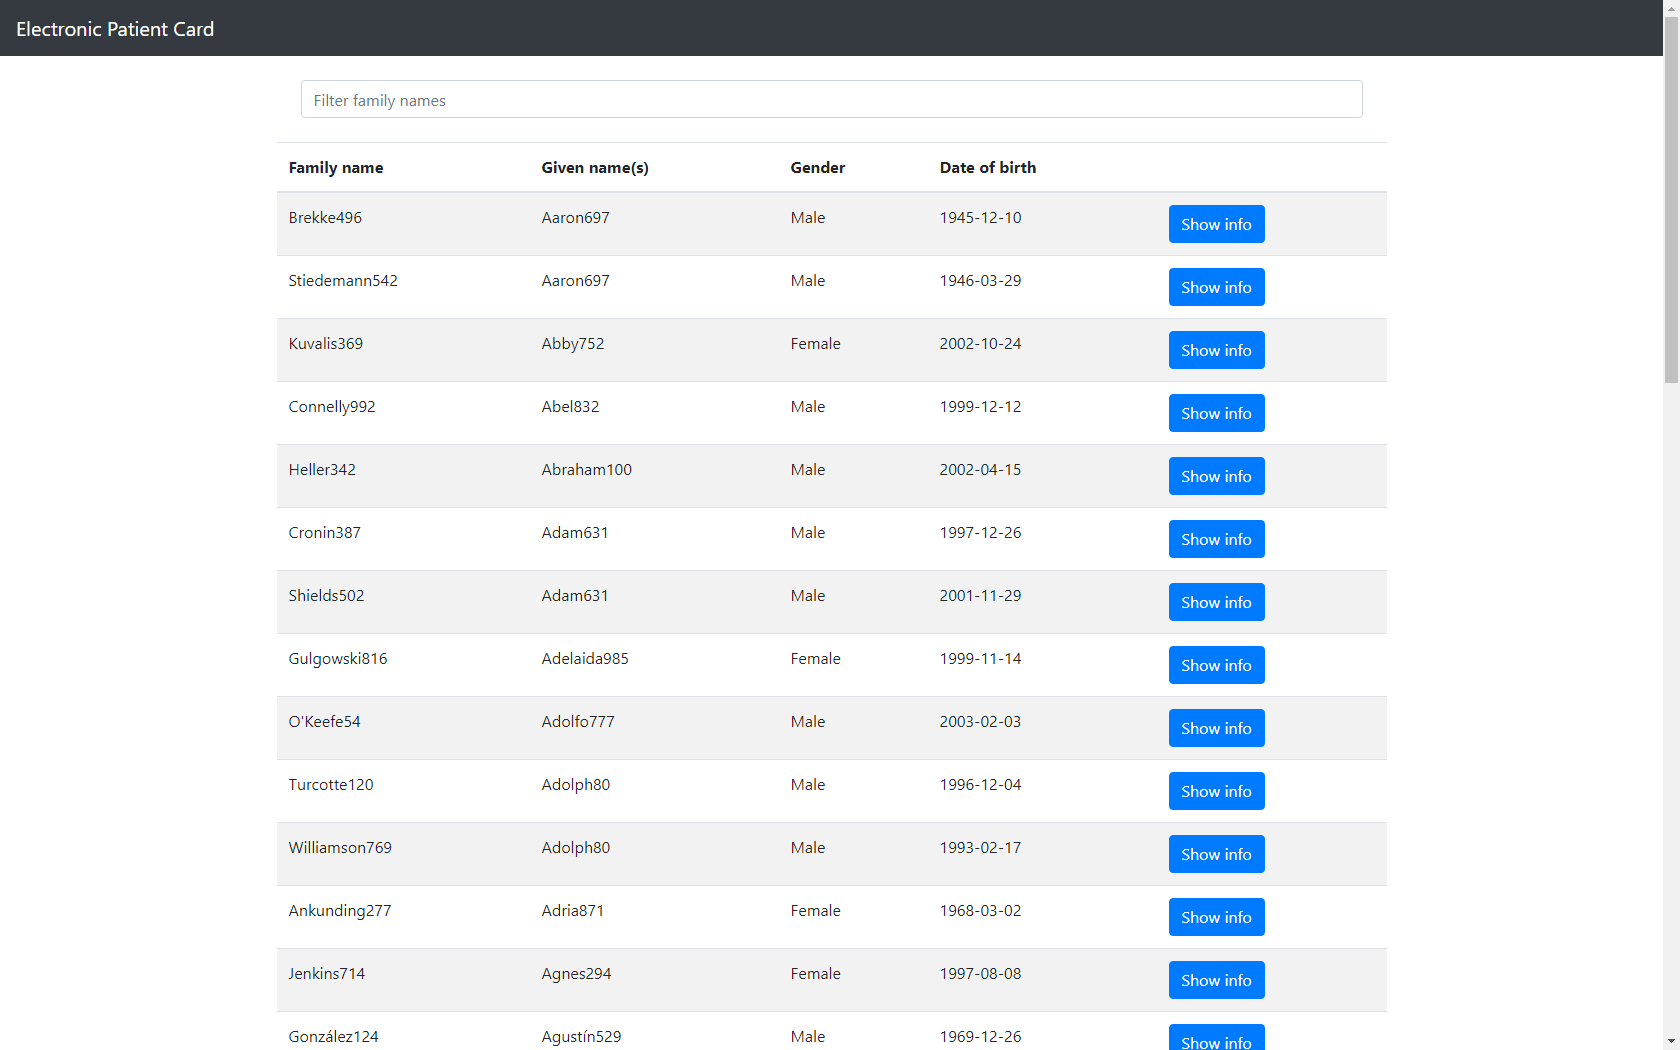
\includegraphics[width=0.8\linewidth]{pic/main_view.PNG}}
    \caption{Lista pacjentów}
\end{figure}

\pagebreak

Użytkownik ma możliwość filtrowania pacjentów po nazwisku. Filtrowanie odbywa się dynamicznie, po każdym 
wprowadzonym znaku lista pacjentów jest aktualizowana tak, aby widniały na niej tylko 
te osoby, w których nazwisku znajduje się wprowadzona fraza.
\begin{figure}[H]
    \center{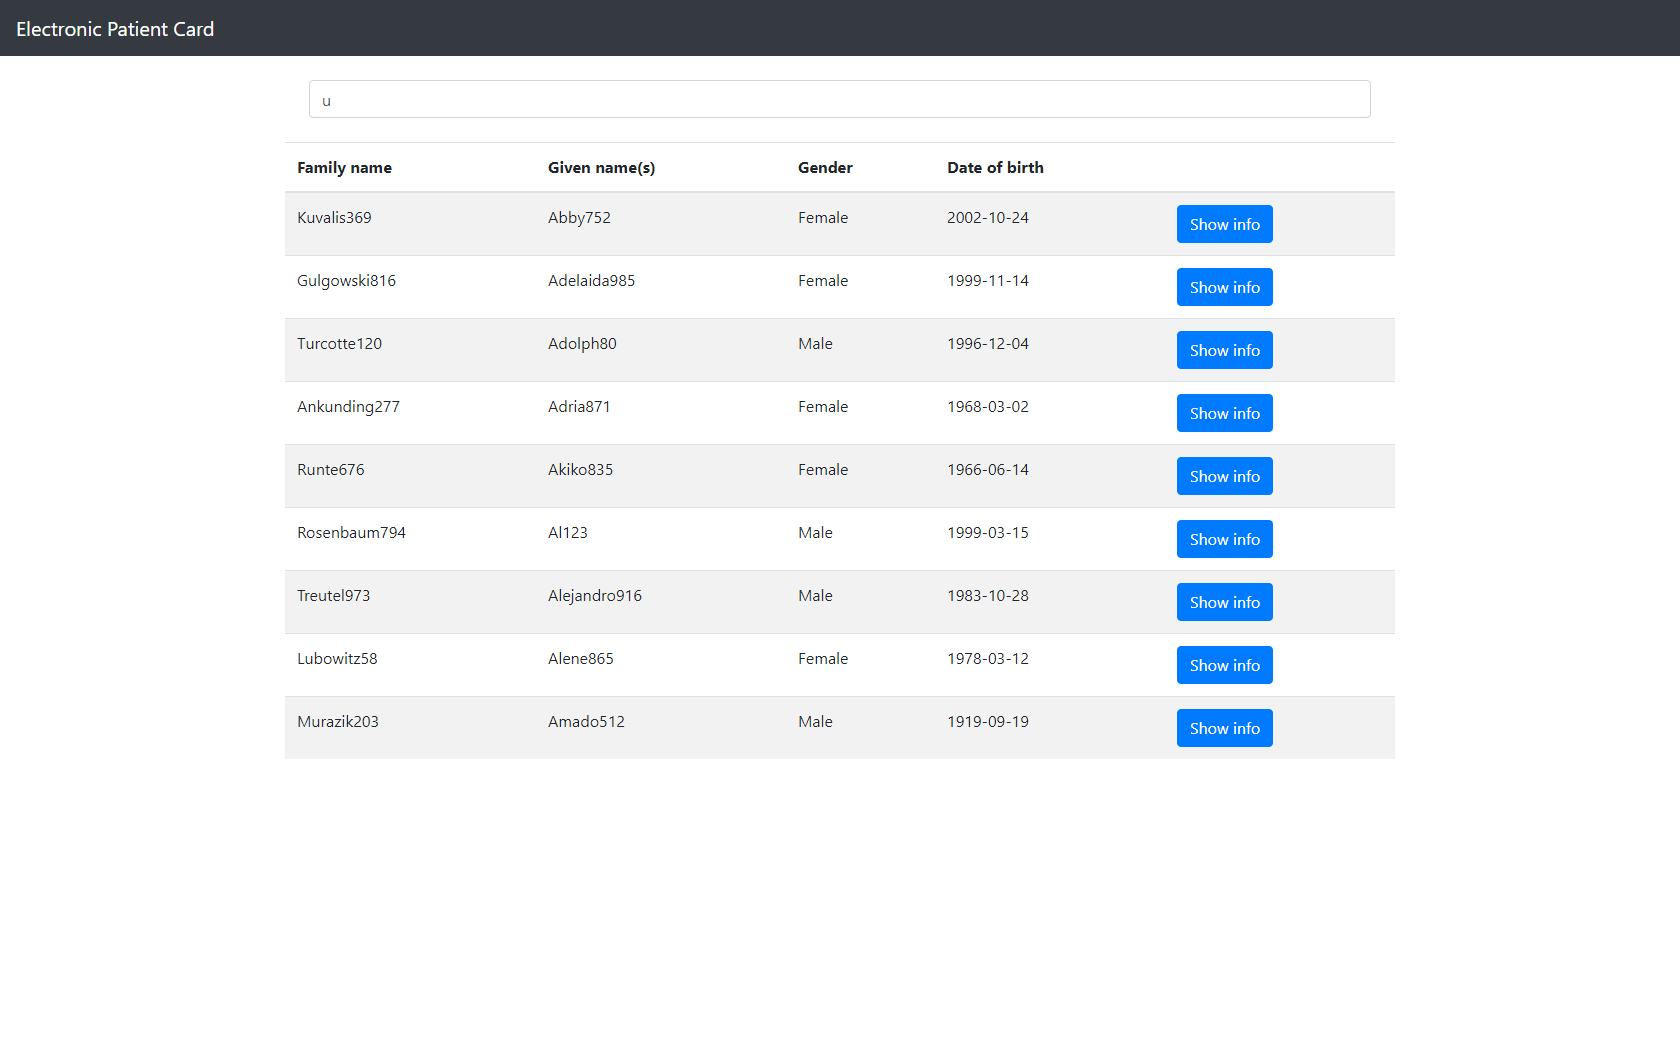
\includegraphics[width=0.8\linewidth]{pic/main_view_filtered.PNG}}
    \caption{Lista pacjentów, których nazwisko zawiera literę \enquote{u}}
\end{figure}

\pagebreak

\section{Informacje na temat pacjenta}
Gdy użytkownik wybierze opcję \enquote{Show info}, z serwera zostaje pobrany pełen zestaw informacji
dotyczących danego pacjenta.
\subsection{Dane personalne}
Główny ekran stanowi wizualizację zasobu \textit{Patient} i jest reprezentacją danych personalnych pacjenta.
\begin{figure}[H]
    \center{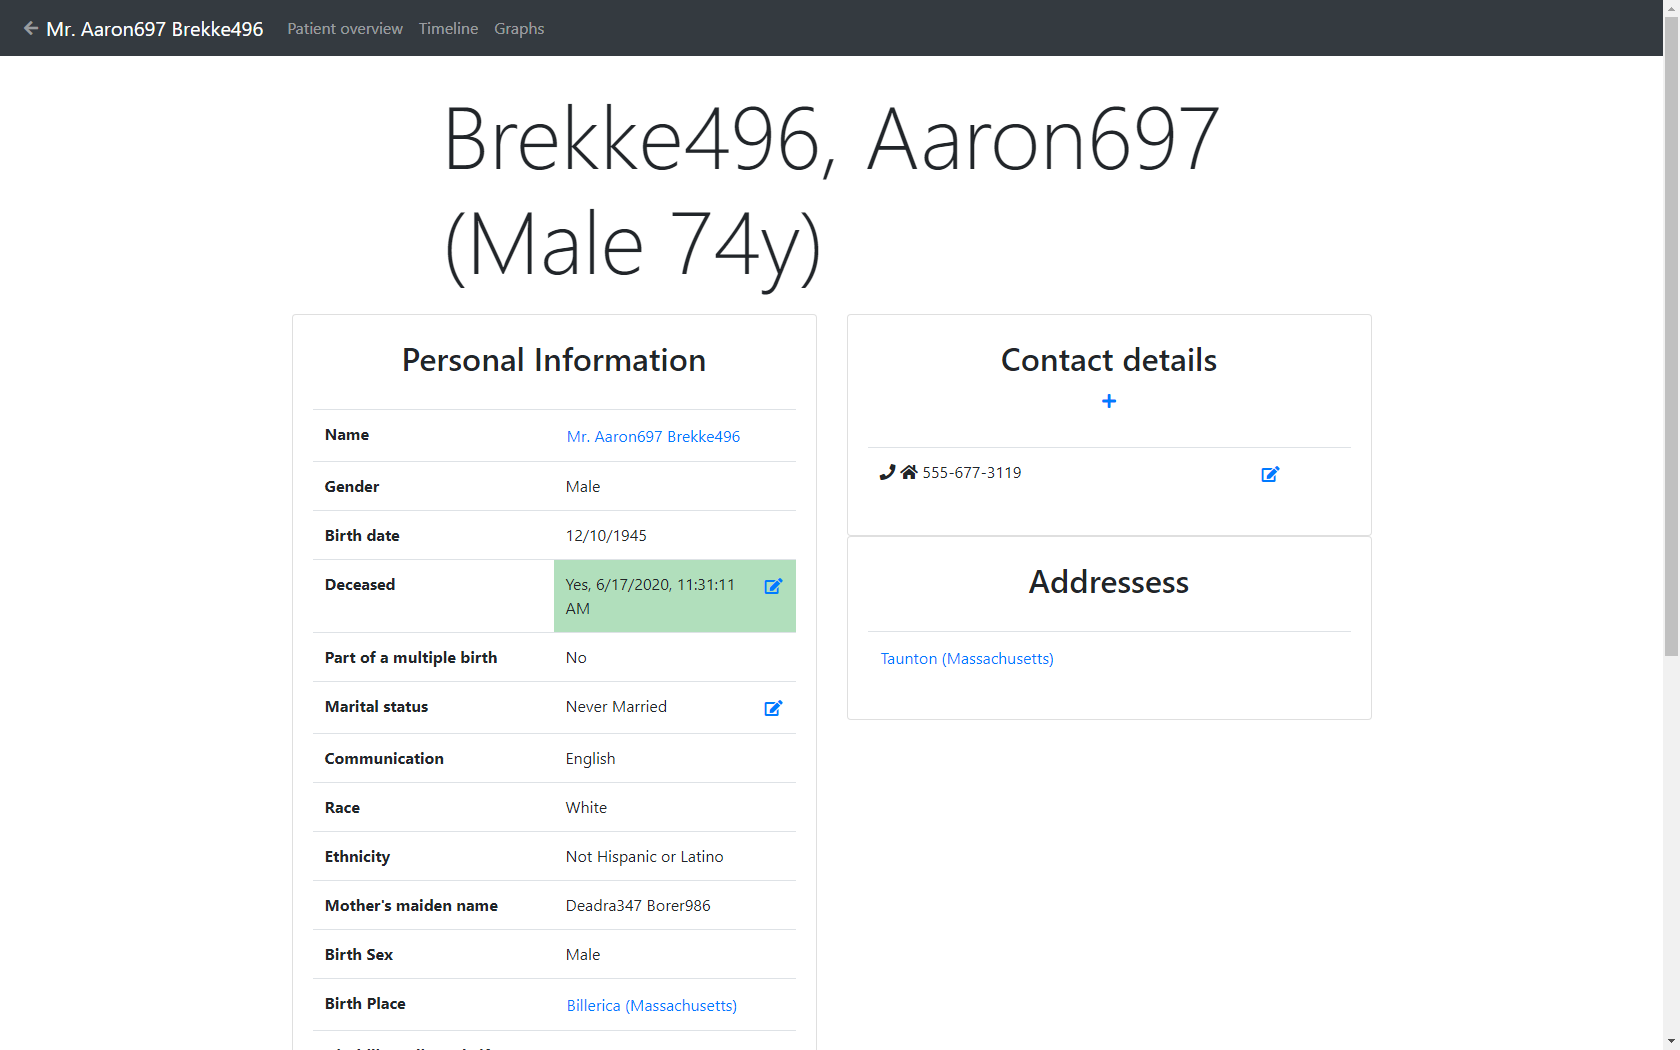
\includegraphics[width=0.8\linewidth]{pic/patient_detail1.PNG}}
    \center{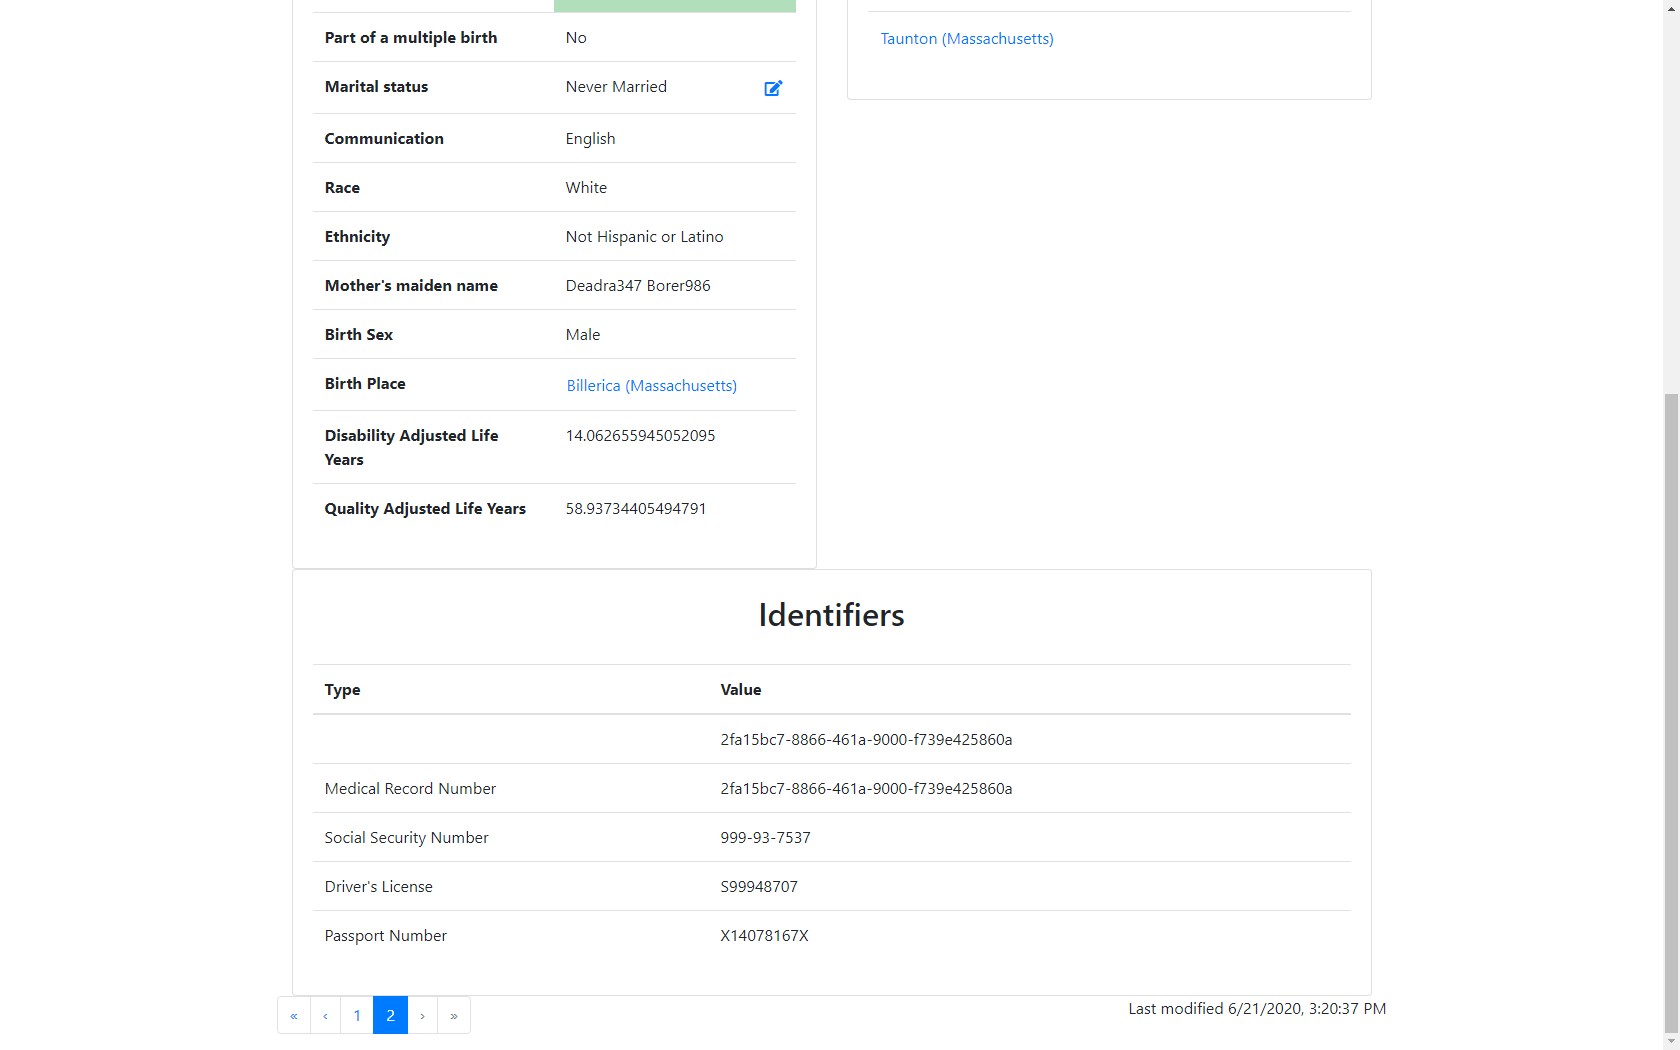
\includegraphics[width=0.8\linewidth]{pic/patient_detail2.PNG}}
    \caption{Dane pacjenta}
\end{figure}

\pagebreak

Dla złożonych zasobów dostępny jest widok szczegółowy. Pola, dla których taki widok jest dostępny wyróżnione są niebieskim tekstem.
\begin{figure}[H]
    \center{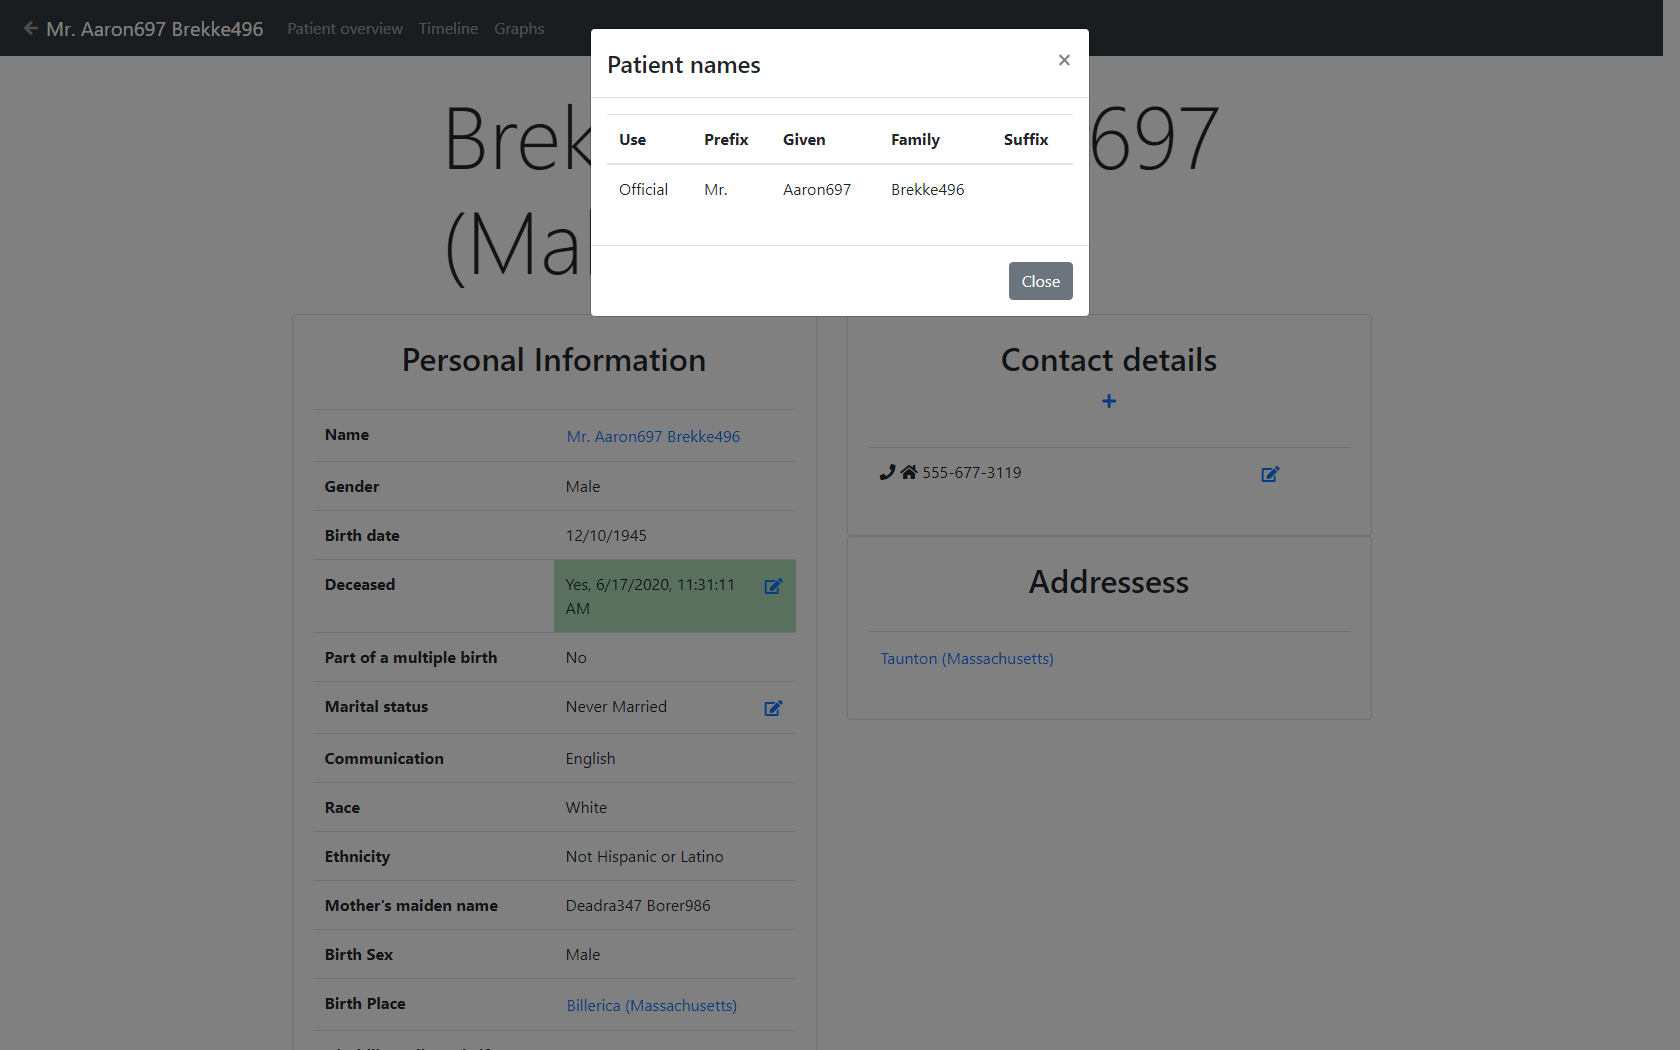
\includegraphics[width=0.8\linewidth]{pic/patient_name_details.PNG}}
    \caption{Wszystkie imiona i nazwiska, którymi posługuje się pacjent}
\end{figure}
\begin{figure}[H]
    \center{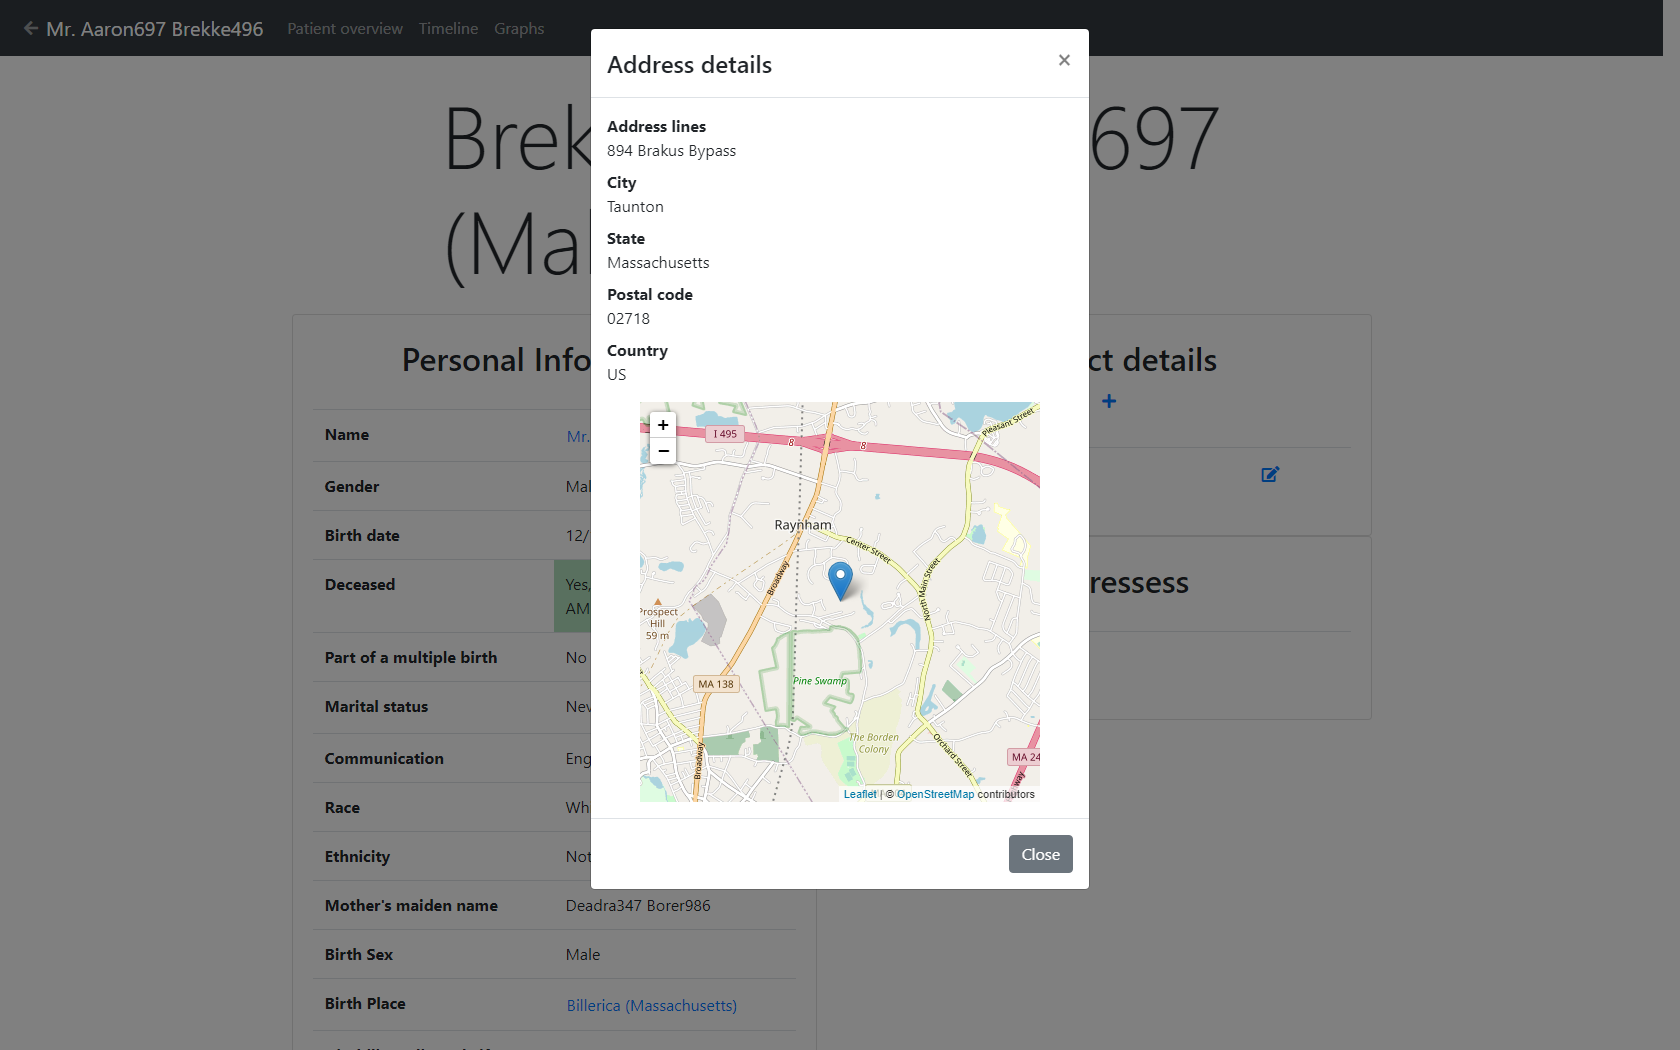
\includegraphics[width=0.8\linewidth]{pic/patient_address_detail.PNG}}
    \caption{Szczegóły dotyczące adresu. Znajdujące się w zasobie współrzędne geograficzne zostały przedstawione na mapie}
\end{figure}

Ponieważ w wykorzystywanej przez nas bazie danych żadne z pól zasobu \textit{Patient}
nie posiada pola \textit{Period}, nie ma w tym widoku możliwości wyboru przedziału czasowego.

\pagebreak

Aplikacja umożliwia modyfikację informacji o stanie cywilnym, zgonie oraz danych kontaktowych pacjenta, jak również dodawanie nowych danych kontaktowych.
\begin{figure}[H]
    \center{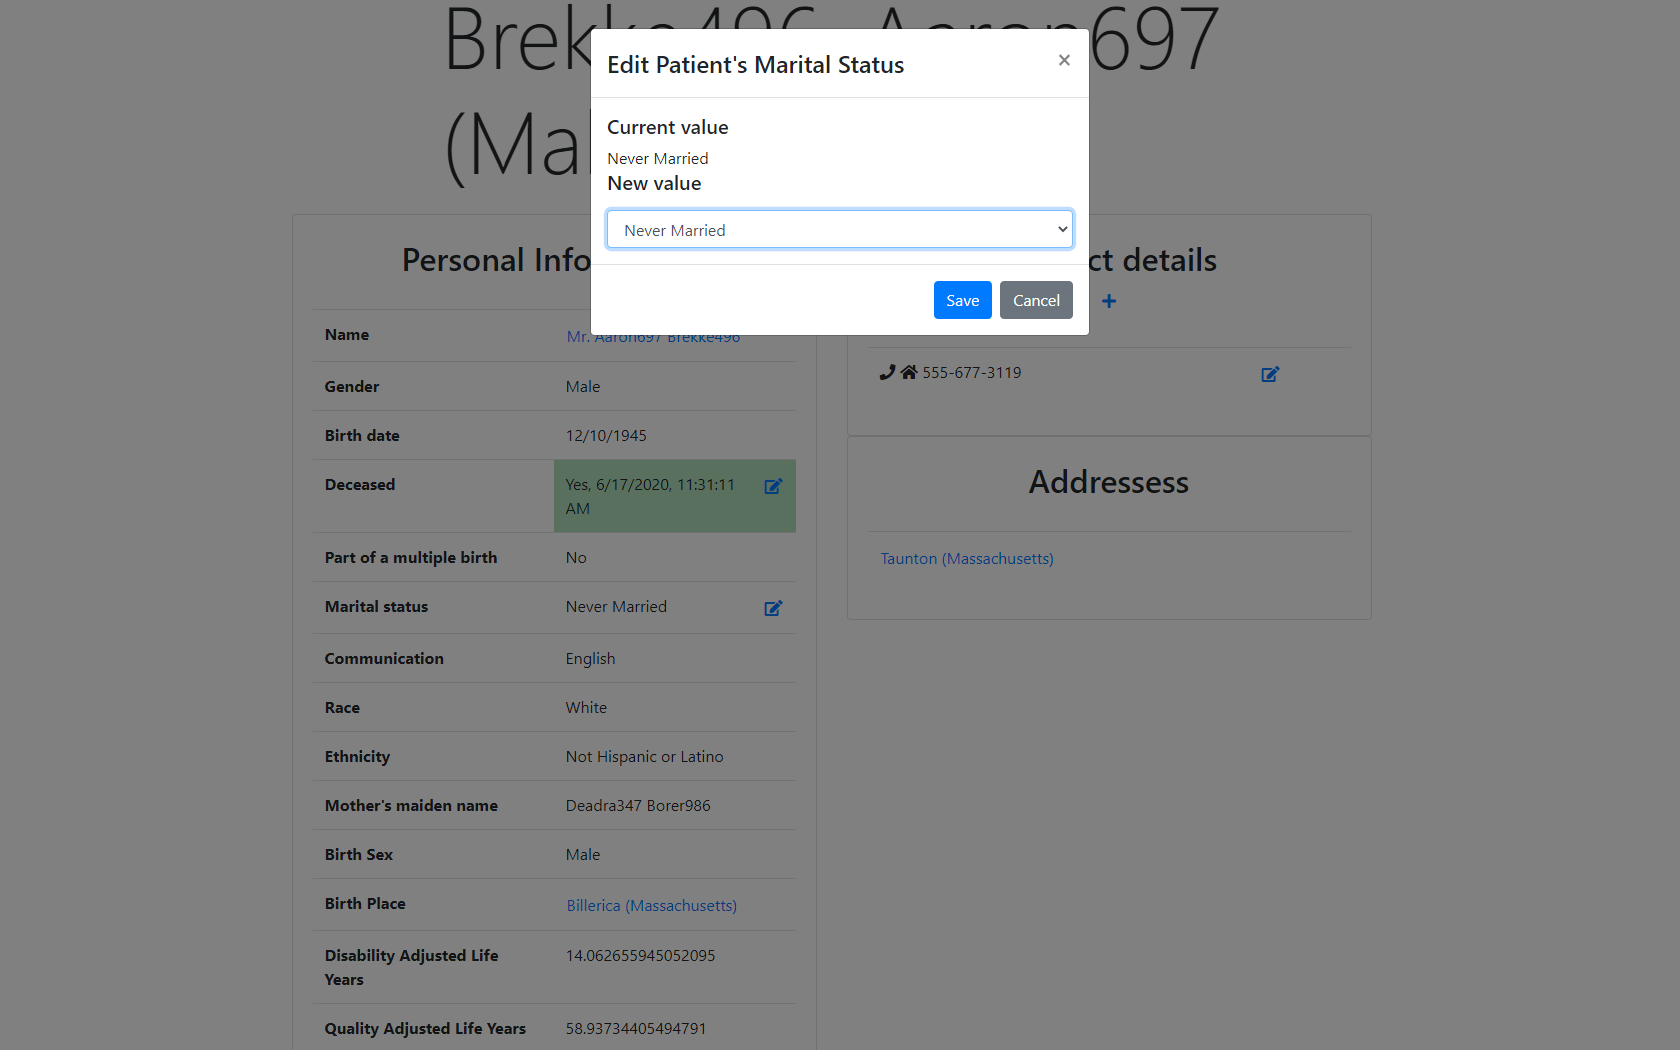
\includegraphics[width=0.8\linewidth]{pic/marital_status_edit.PNG}}
    \center{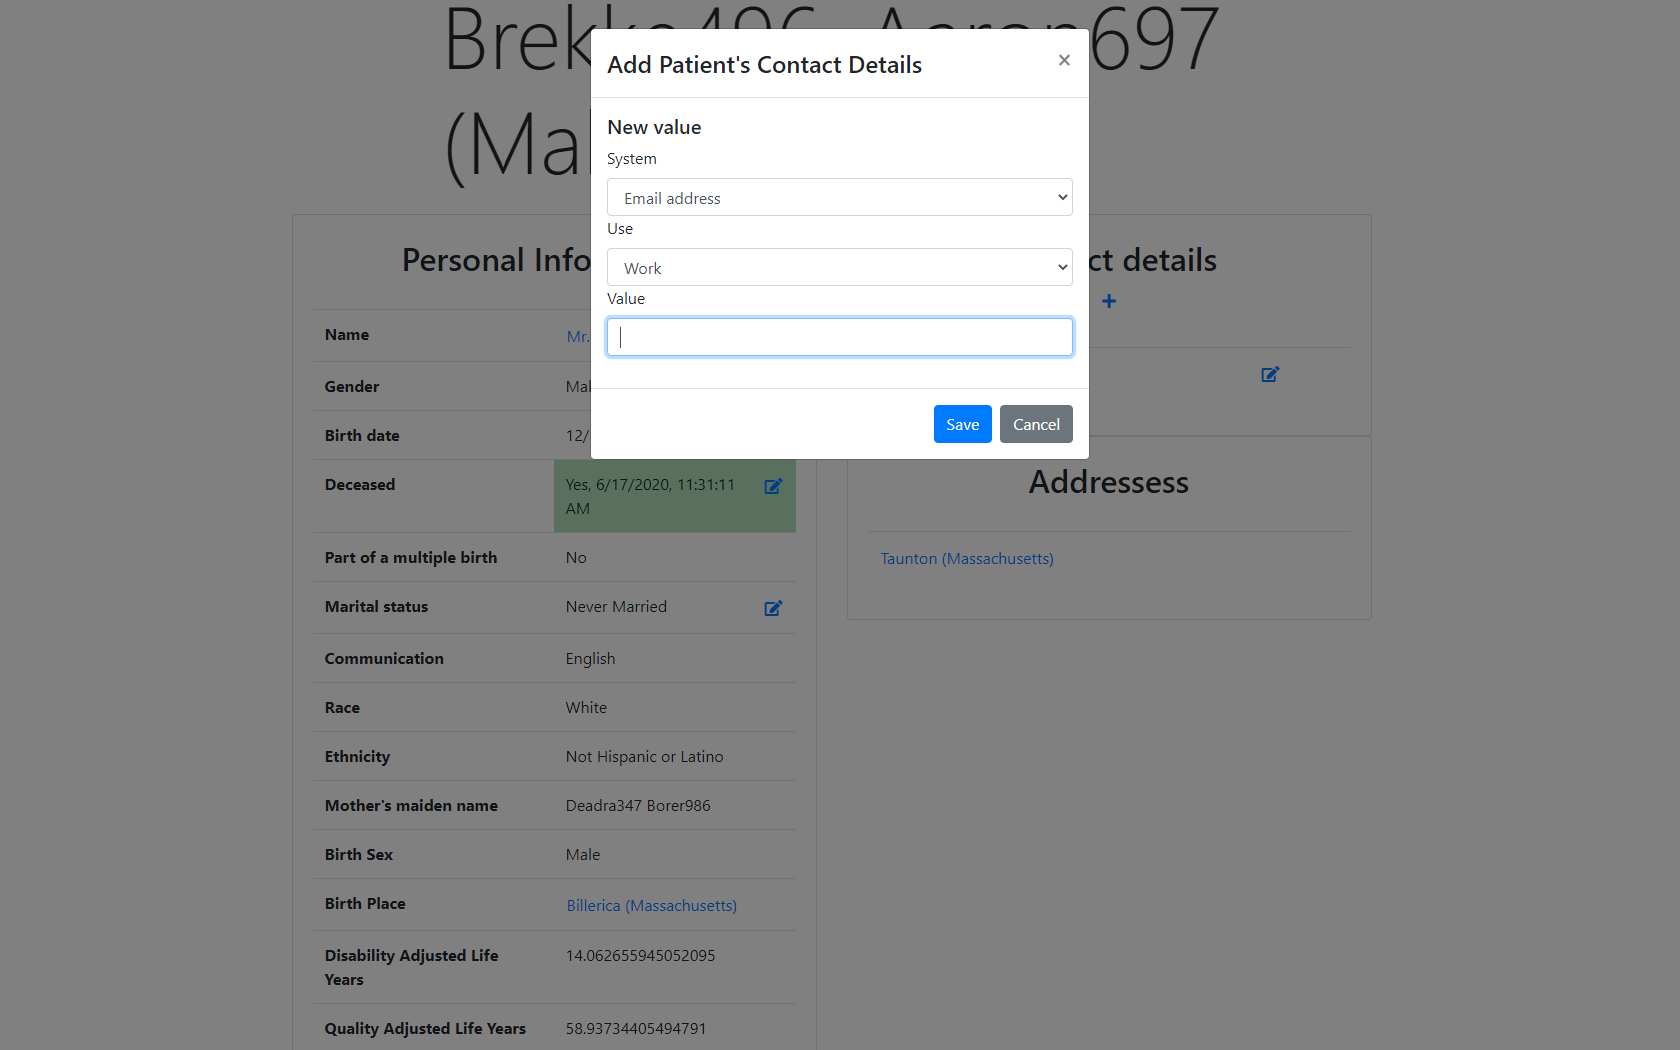
\includegraphics[width=0.8\linewidth]{pic/add_contact_details.PNG}}
    \caption{Widok edycji stanu cywilnego i dodawania metody kontaktu}
\end{figure}

Aplikacja informuje użytkownika o dostępności innych wersji zasobu i umożliwia przechodzenie między nimi 
za pomocą przycisków znajdujących się u dołu ekranu. Wyświetla również informację o dacie modyfikacji.
Pola, które w stosunku do poprzedniej wersji uległy zmianie są wyróżnione kolorem zielonym.
Ta funkcjonalność została zaprezentowana na rysunku 3.

\subsection{Oś czasu}
Na osi czasu przedstawione są zasoby \textit{MedicationRequest} oraz \textit{Observation}.
Użytkownik może poruszać się po osi czasu za pomocą myszy.
\begin{figure}[H]
    \center{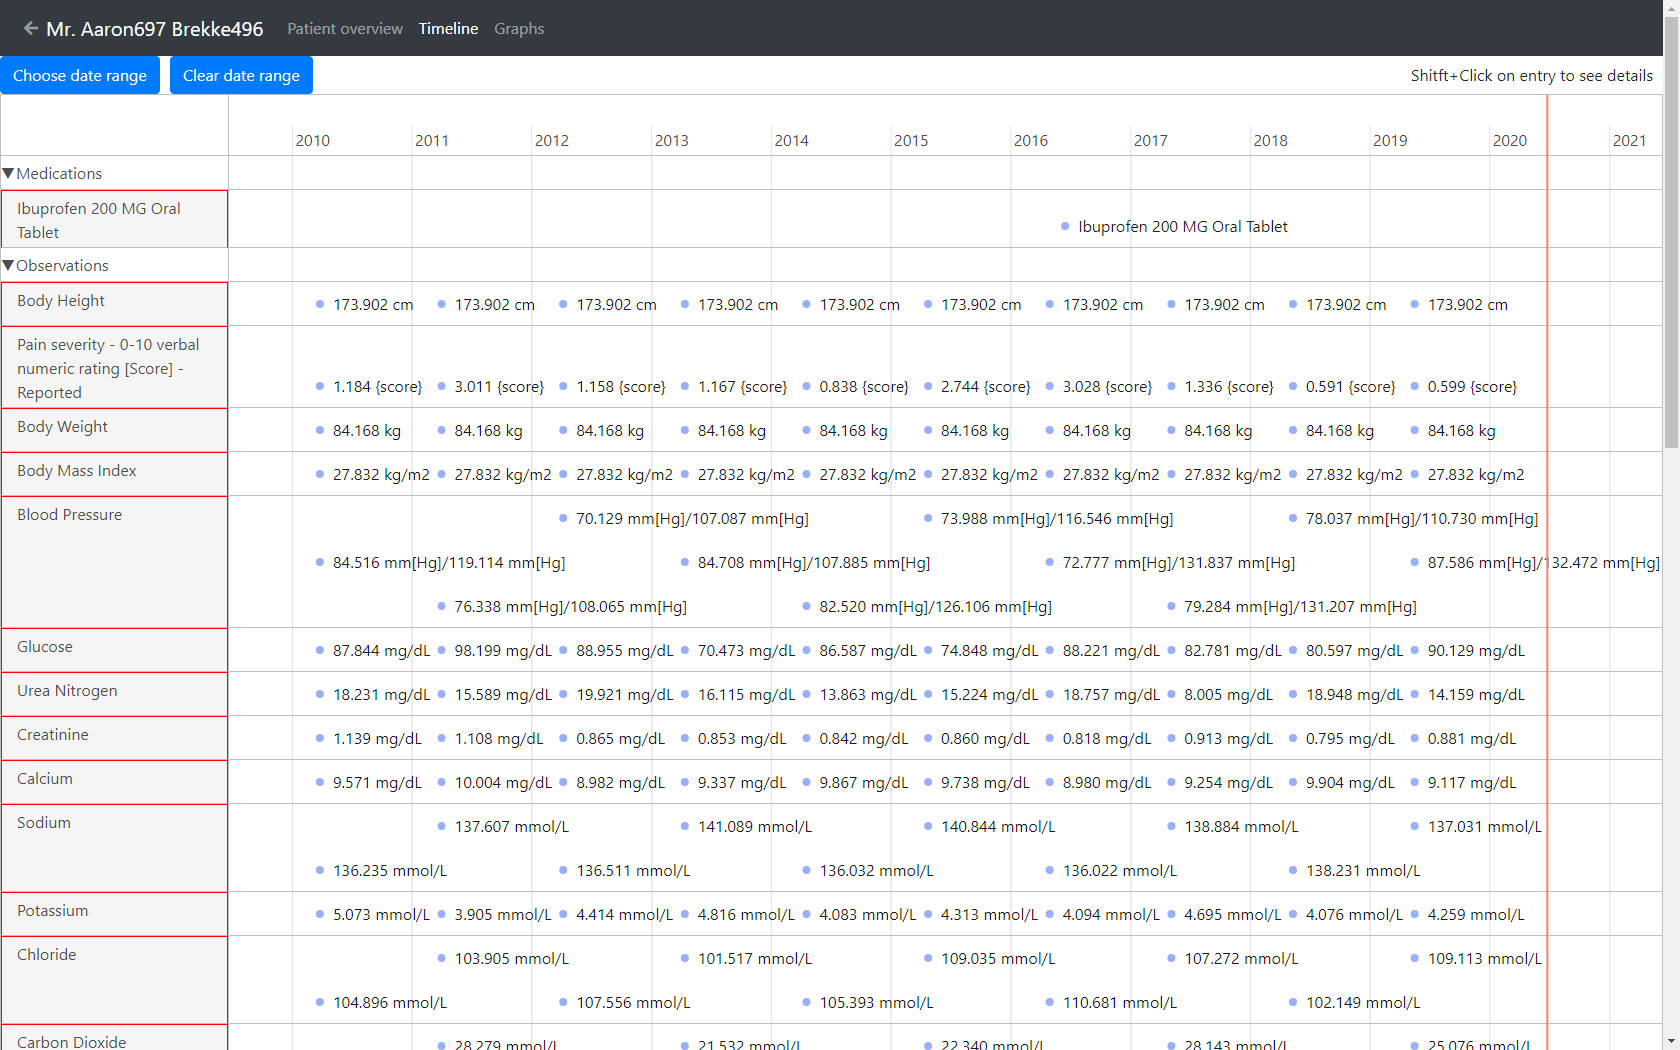
\includegraphics[width=0.8\linewidth]{pic/timeline.PNG}}
    \caption{Oś czasu}
\end{figure}

Dodatkowo, użytkownik może filtrować wizualizowane zasoby poprzez sprecyzowanie okresu.
\begin{figure}[H]
    \center{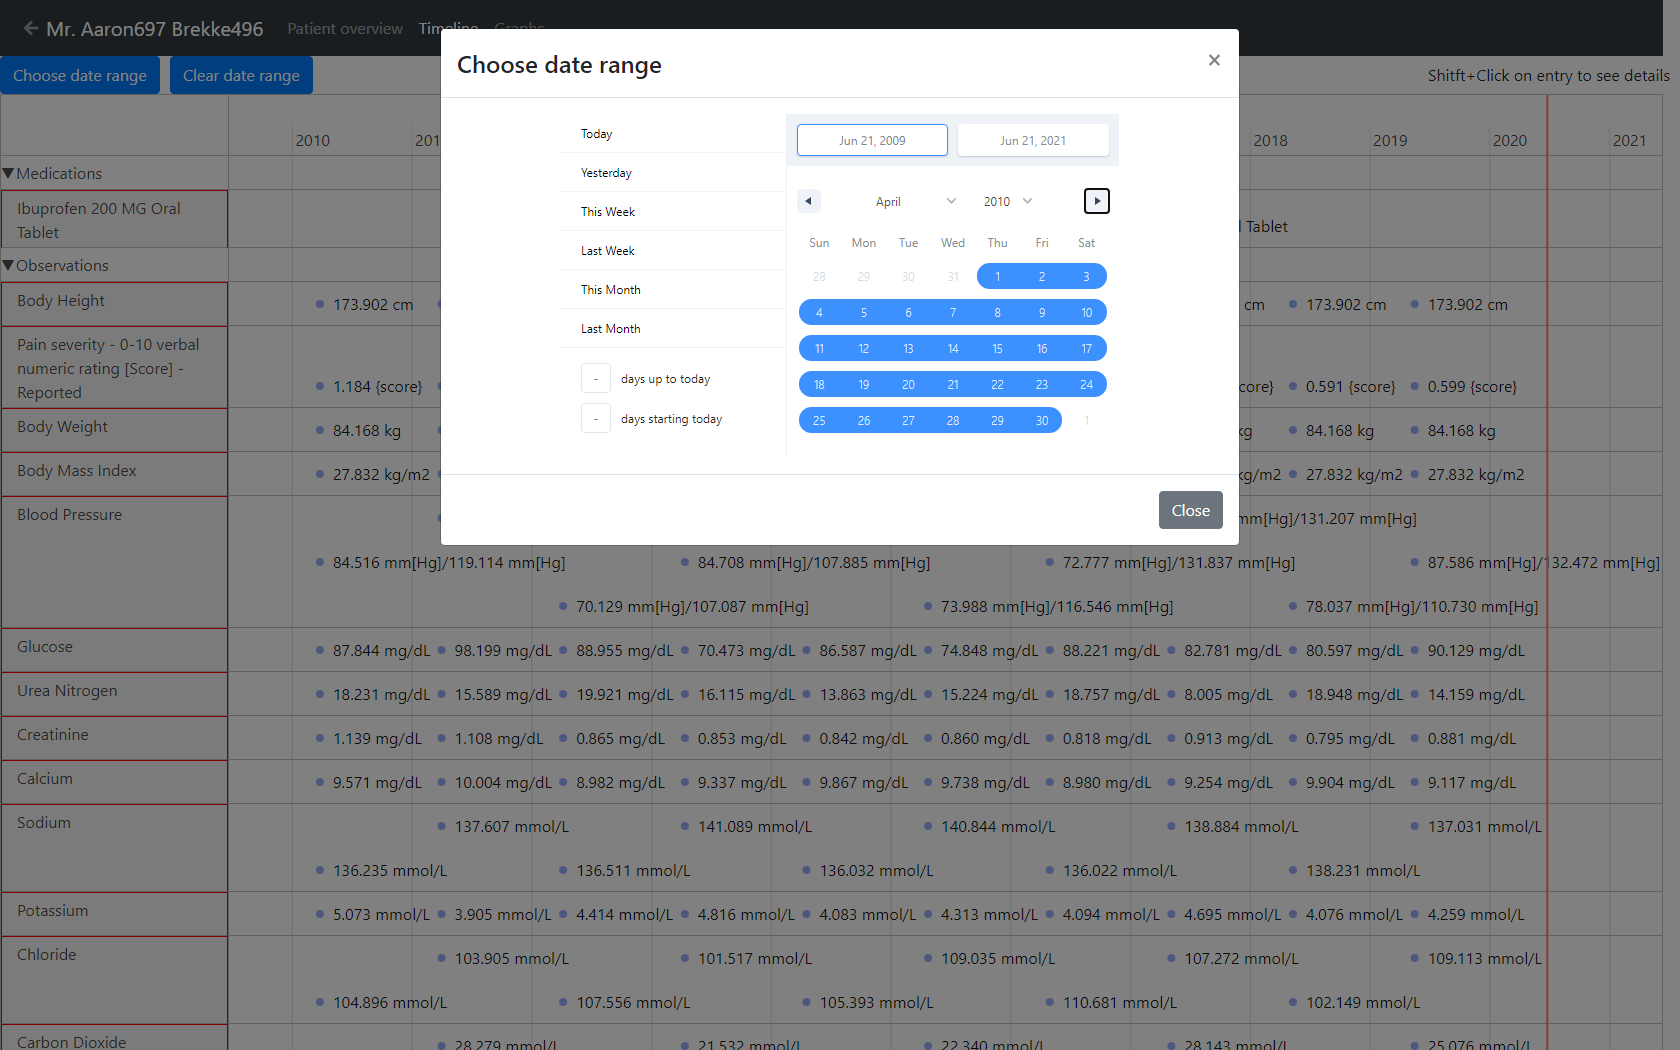
\includegraphics[width=0.8\linewidth]{pic/timeline_date_range.PNG}}
    \caption{Precyzowanie okresu}
\end{figure}

\pagebreak

Po wybraniu pozycji na osi (kliknięcie z wciśniętym przyciskiem Shift) użytkownik może zapoznać się ze szczegółowymi 
informacjami dotyczącymi wybranego zasobu.
\begin{figure}[H]
    \center{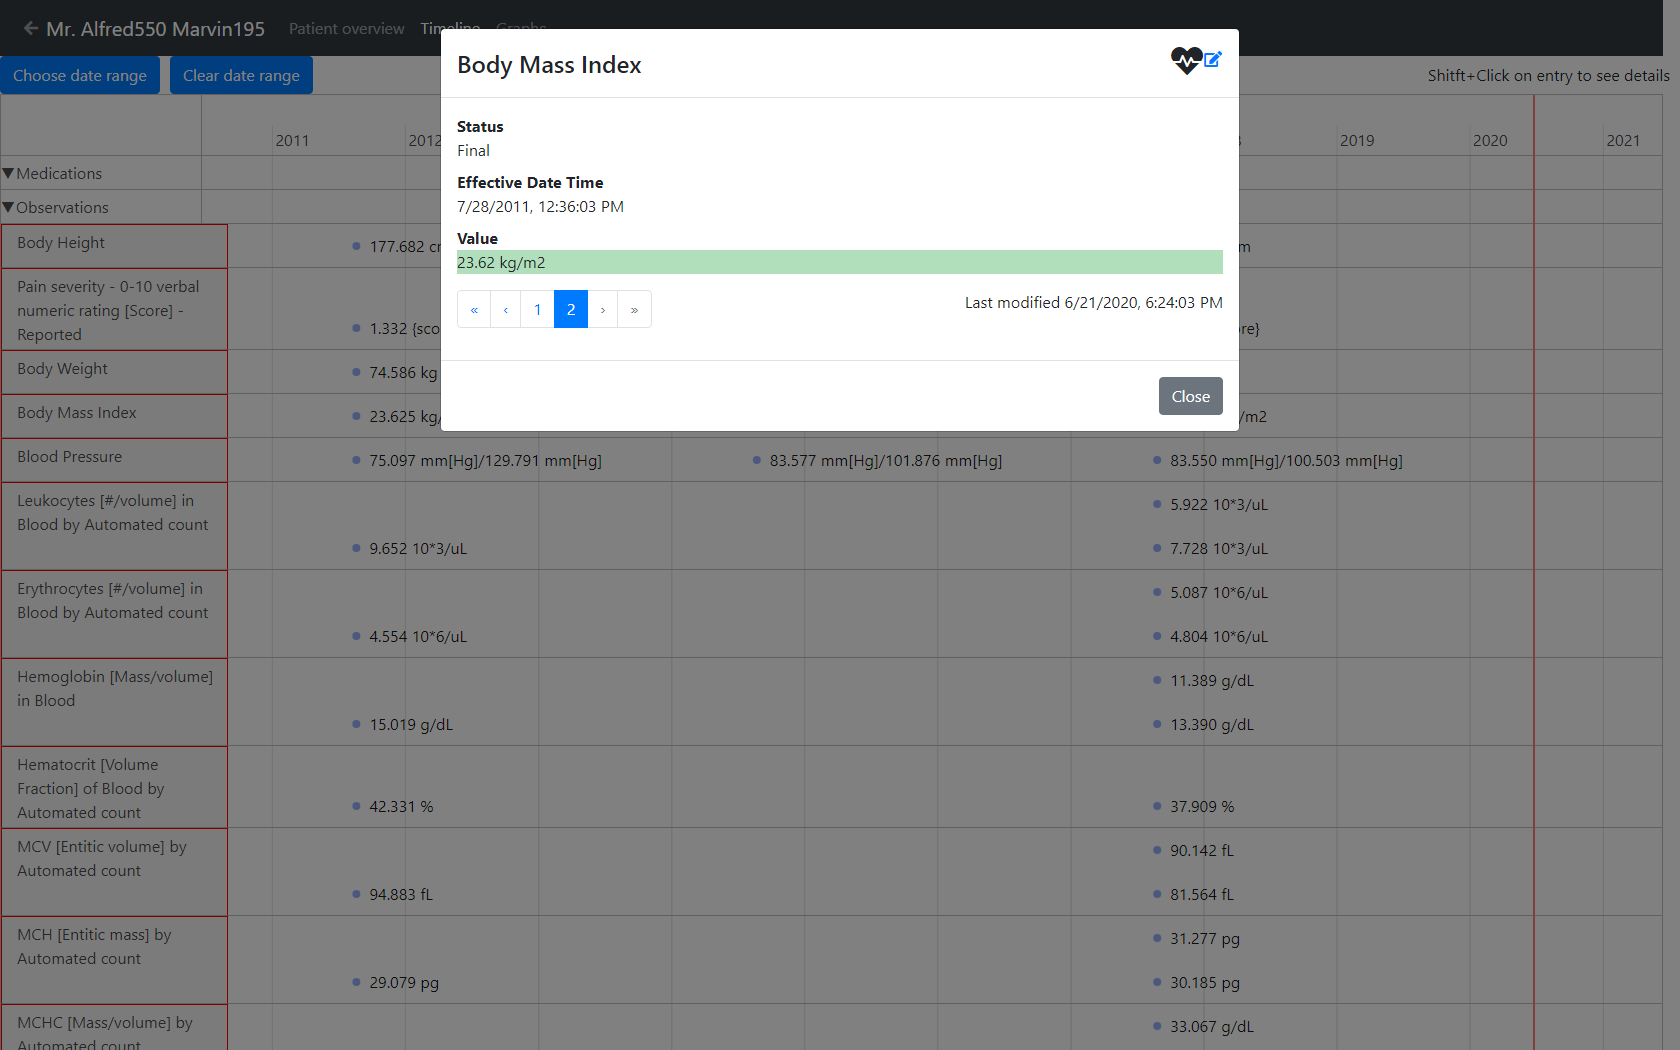
\includegraphics[width=0.8\linewidth]{pic/observation_details.PNG}}
    \center{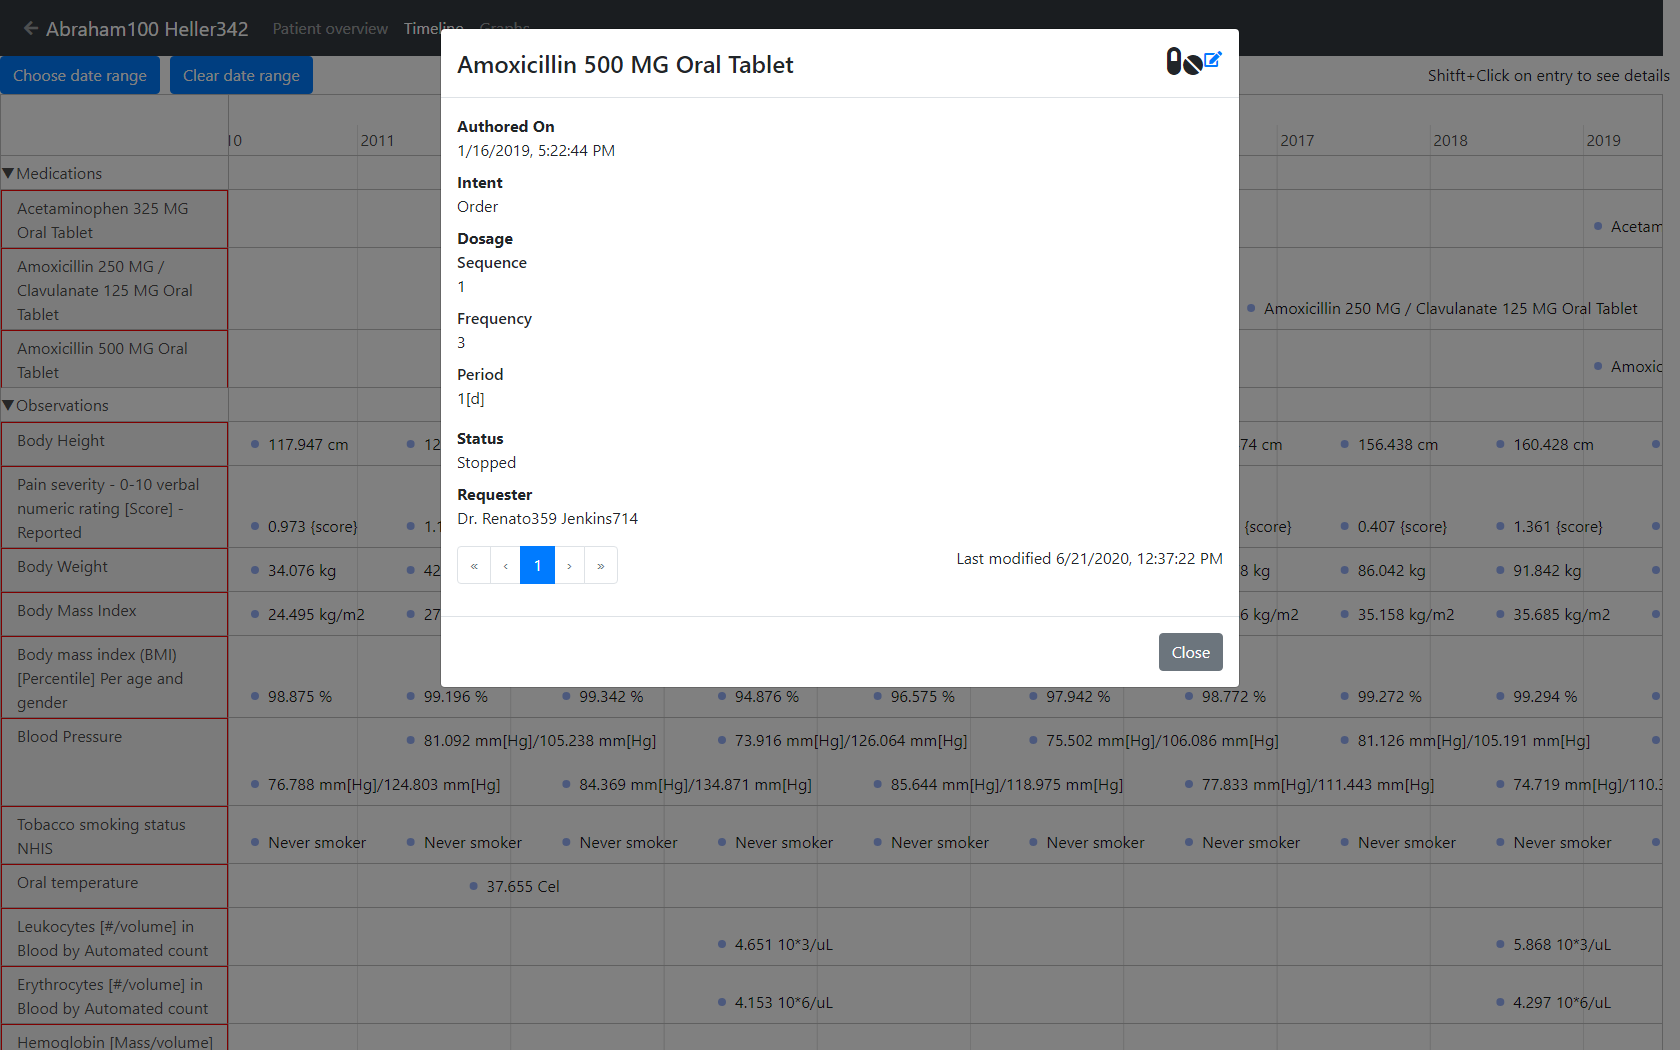
\includegraphics[width=0.8\linewidth]{pic/medication_request_details.PNG}}
    \caption{Szczegóły zasobu}
\end{figure}

\pagebreak

Dla każdej obserwacji użytkownik może dokonać edycji stanu, daty oraz wartości liczbowej - zarówno pojedynczej, jak i złożonej (np. ciśnienie tętnicze).
\begin{figure}[H]
    \center{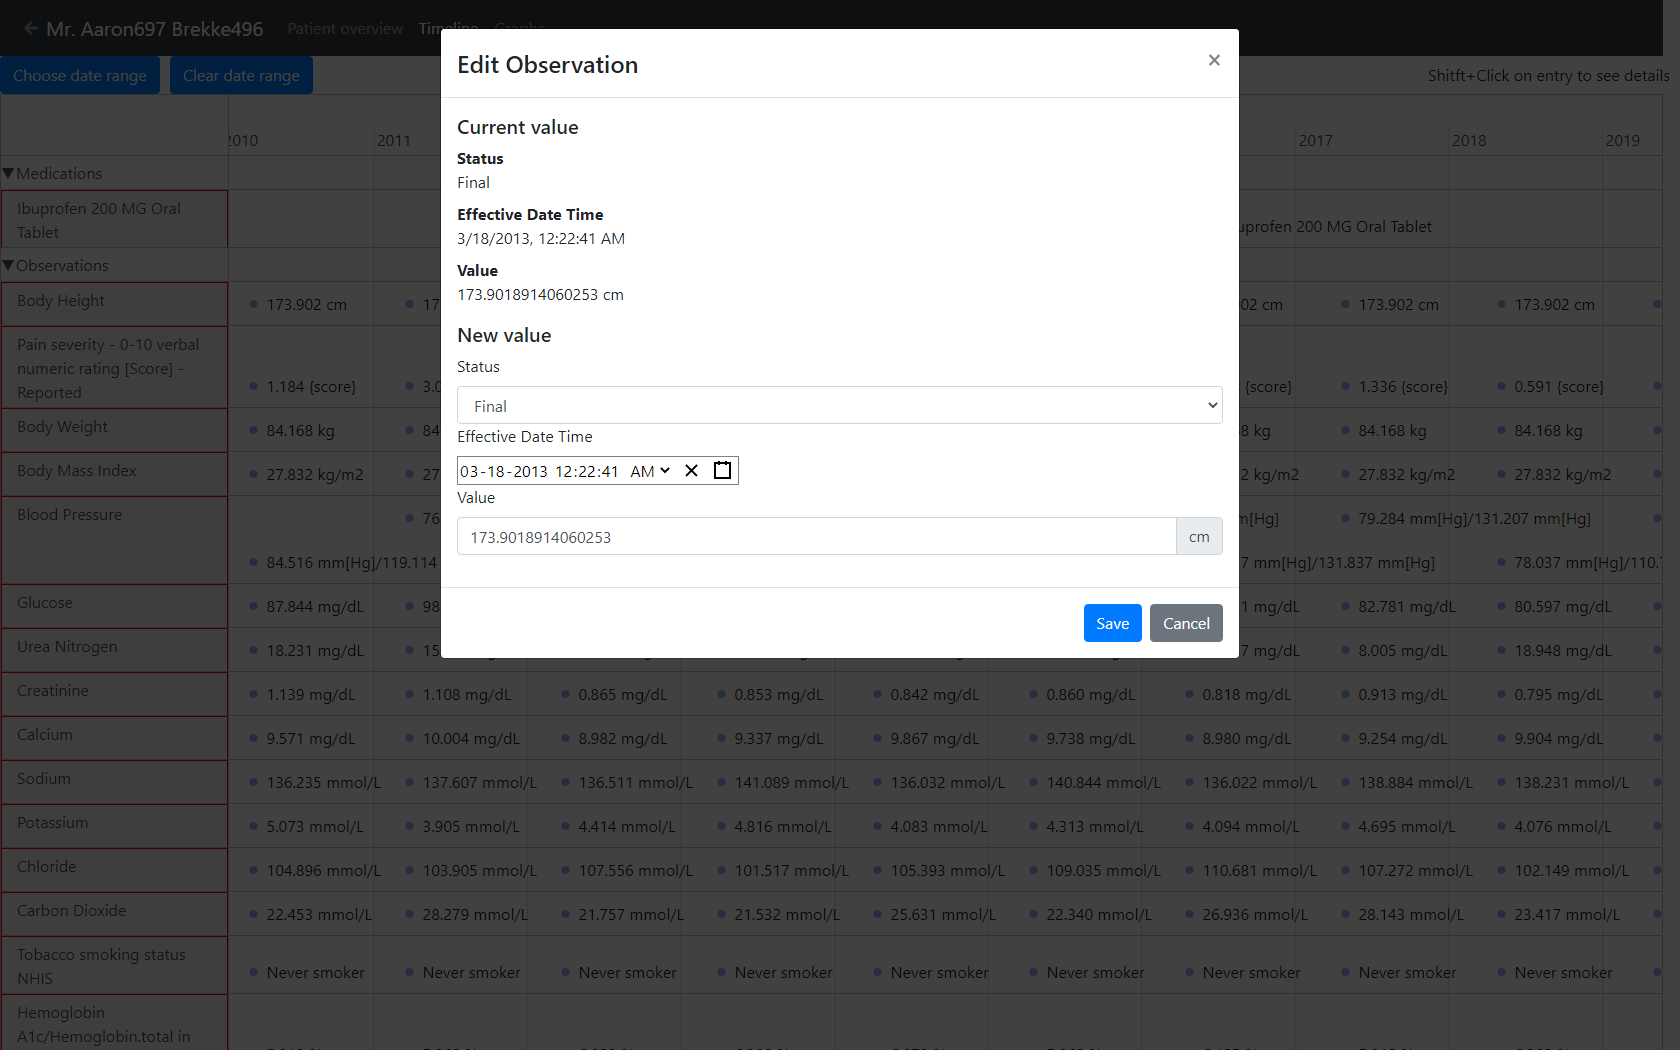
\includegraphics[width=0.8\linewidth]{pic/observation_edit.PNG}}
    \center{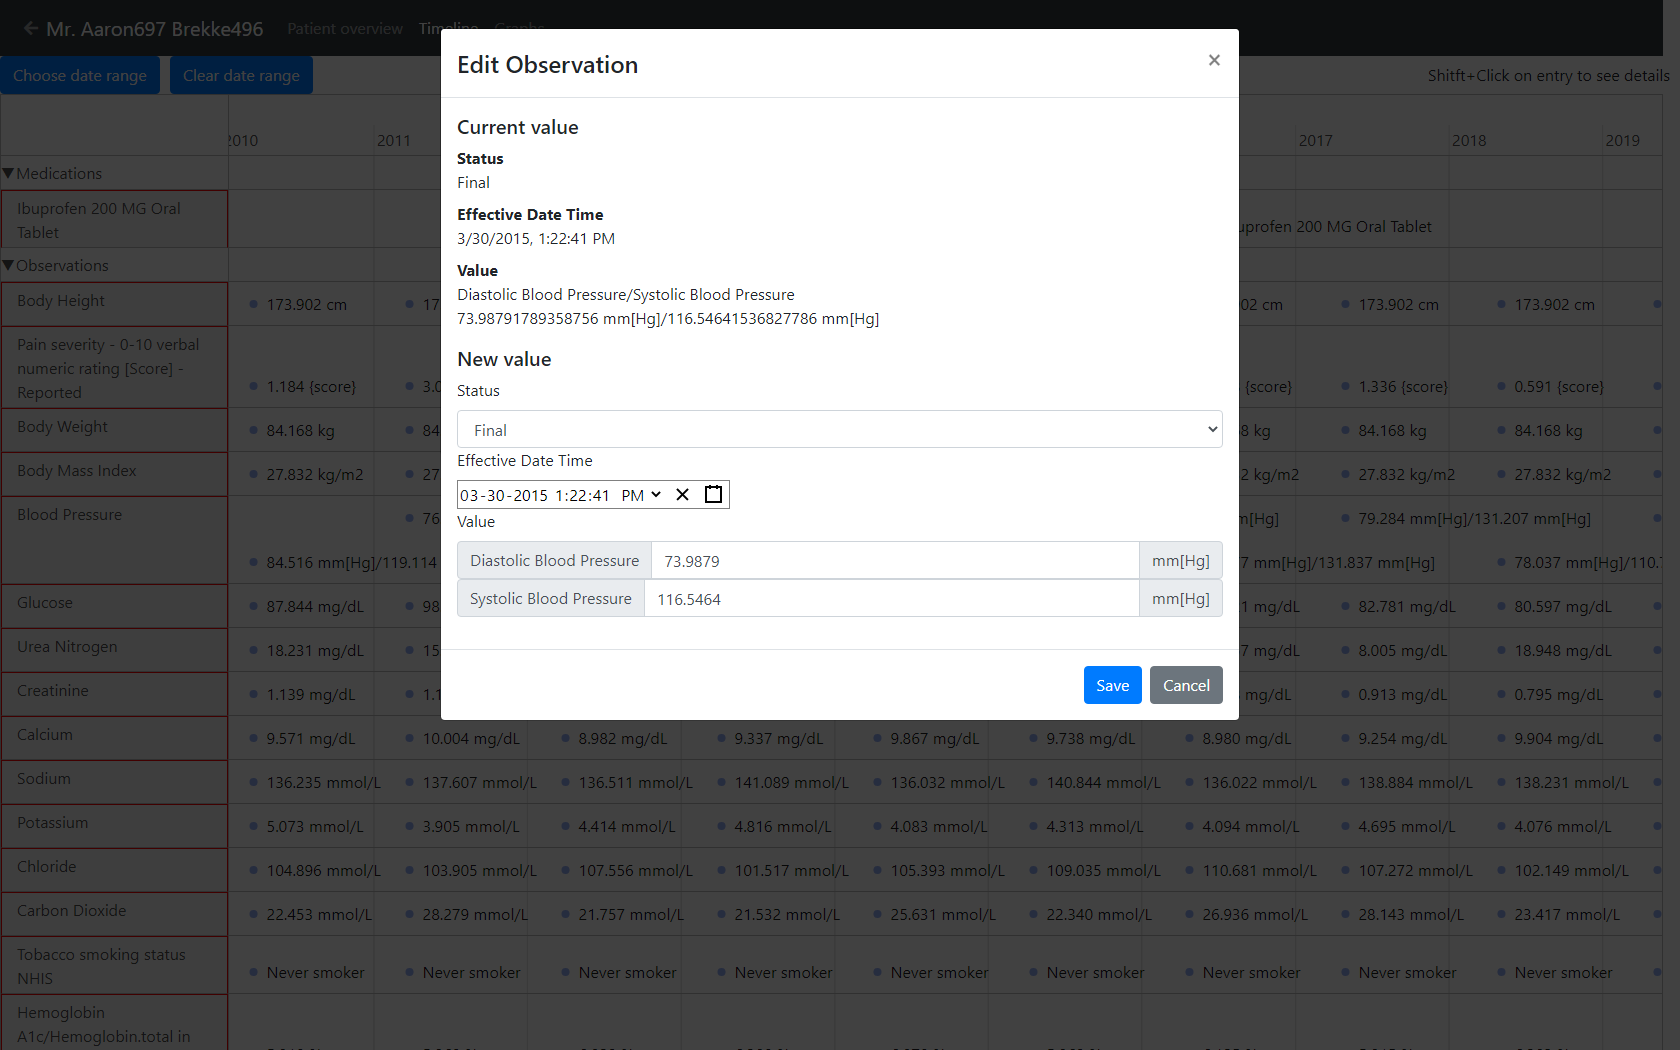
\includegraphics[width=0.8\linewidth]{pic/observation_edit_complex.PNG}}
    \caption{Edycja obserwacji}
\end{figure}

\pagebreak

Dla każdego zasobu \textit{MedicationRequest} użytkownik może dokonać edycji stanu, daty wystawienia oraz typu - czy jest to plan, zalecenie, itd.
\begin{figure}[H]
    \center{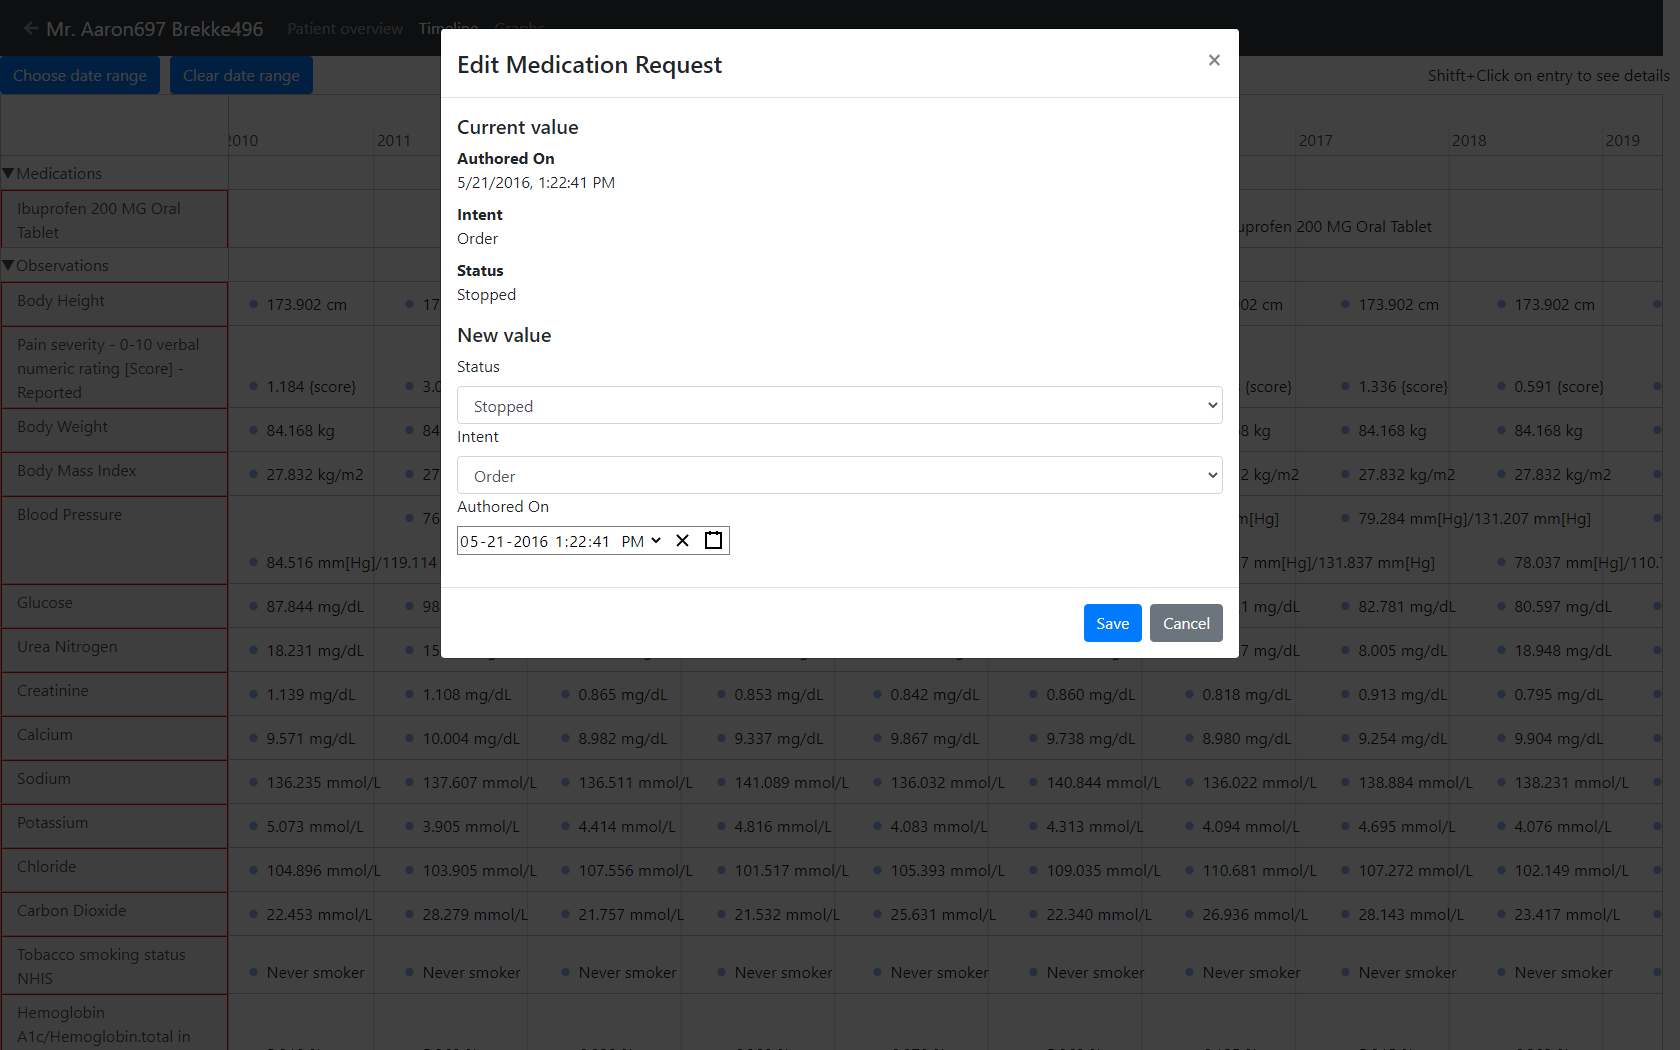
\includegraphics[width=0.8\linewidth]{pic/medication_request_edit.PNG}}
    \center{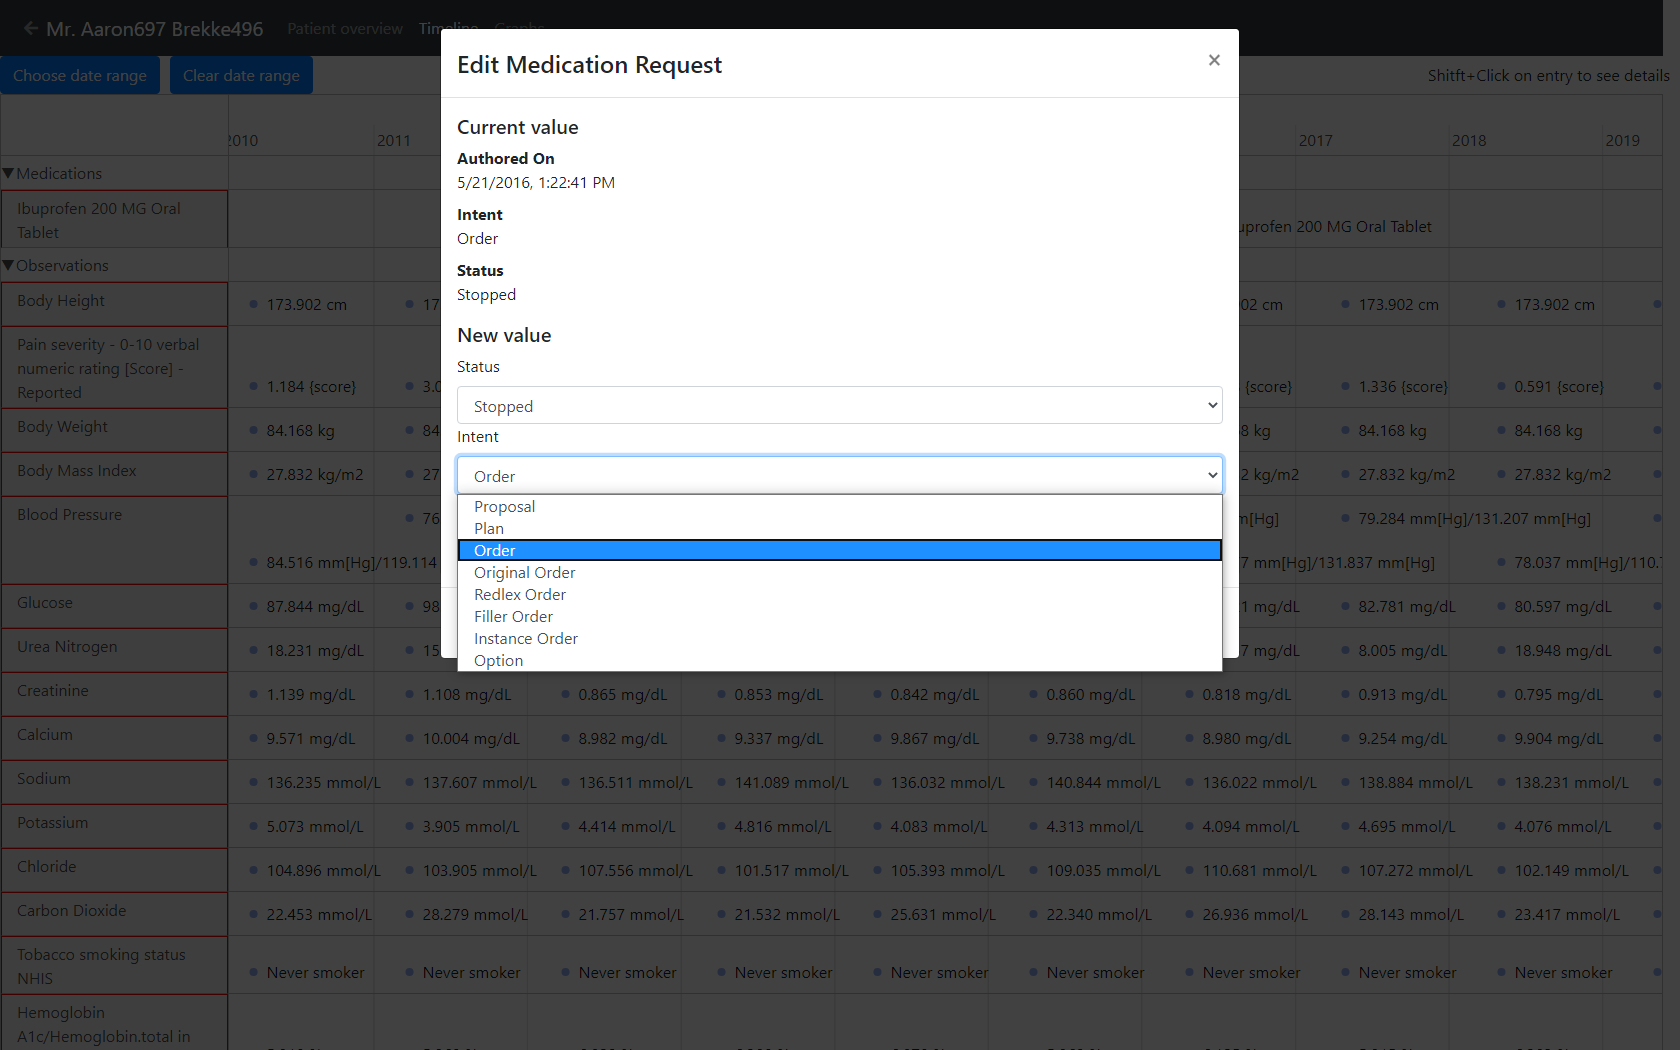
\includegraphics[width=0.8\linewidth]{pic/medication_request_edit2.PNG}}
    \caption{Edycja \textit{MedicationRequest}}
\end{figure}

\pagebreak

Podobnie jak w przypadku zasobu \textit{Patient} każde okienko ze szczegółami informuje użytkownika o dostępnych wersjach, dacie ostatniej zmiany i polach, które
uległy zmianie względem wcześniejszej wersji.
\begin{figure}[H]
    \center{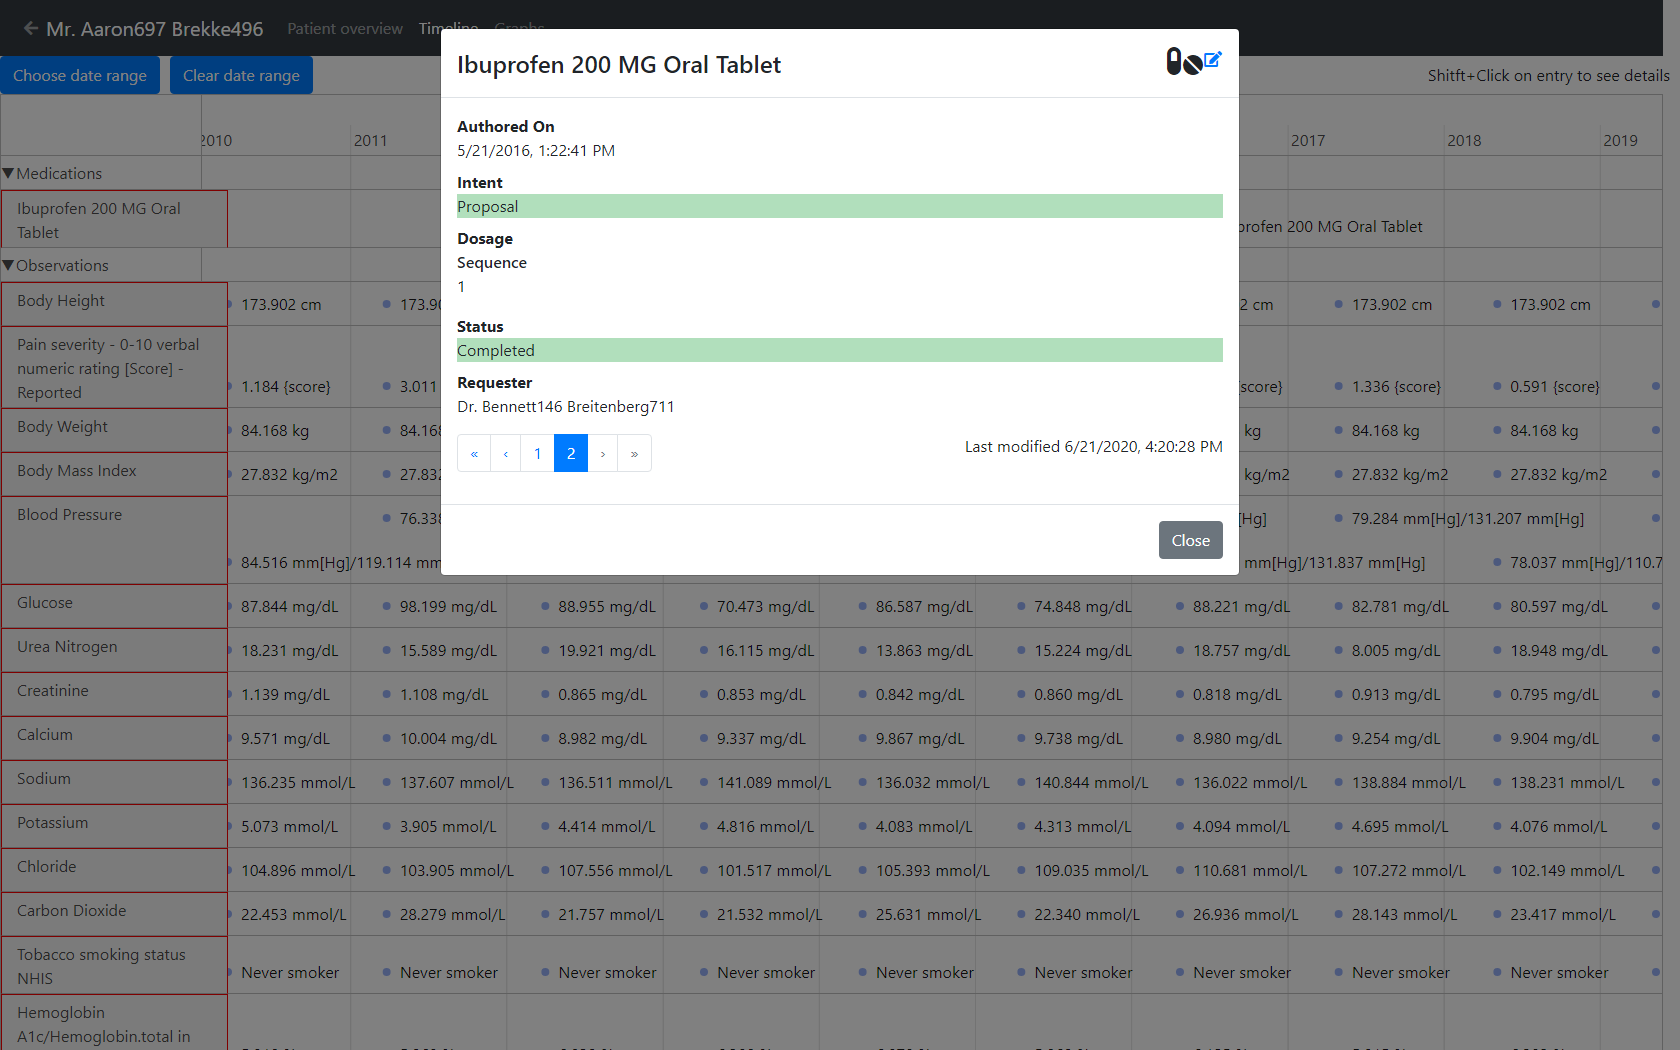
\includegraphics[width=0.8\linewidth]{pic/medication_request_history.PNG}}
    \caption{Zmiany względem poprzedniej wersji}
\end{figure}

\subsection{Wykres}
Aplikacja umożliwia przedstawienie na wykresie dowolnych obserwacji, które posiadają pojedynczą wartość liczbową,
tj. mają zdefiniowane pole \textit{valueQuantity}.
\begin{figure}[H]
    \center{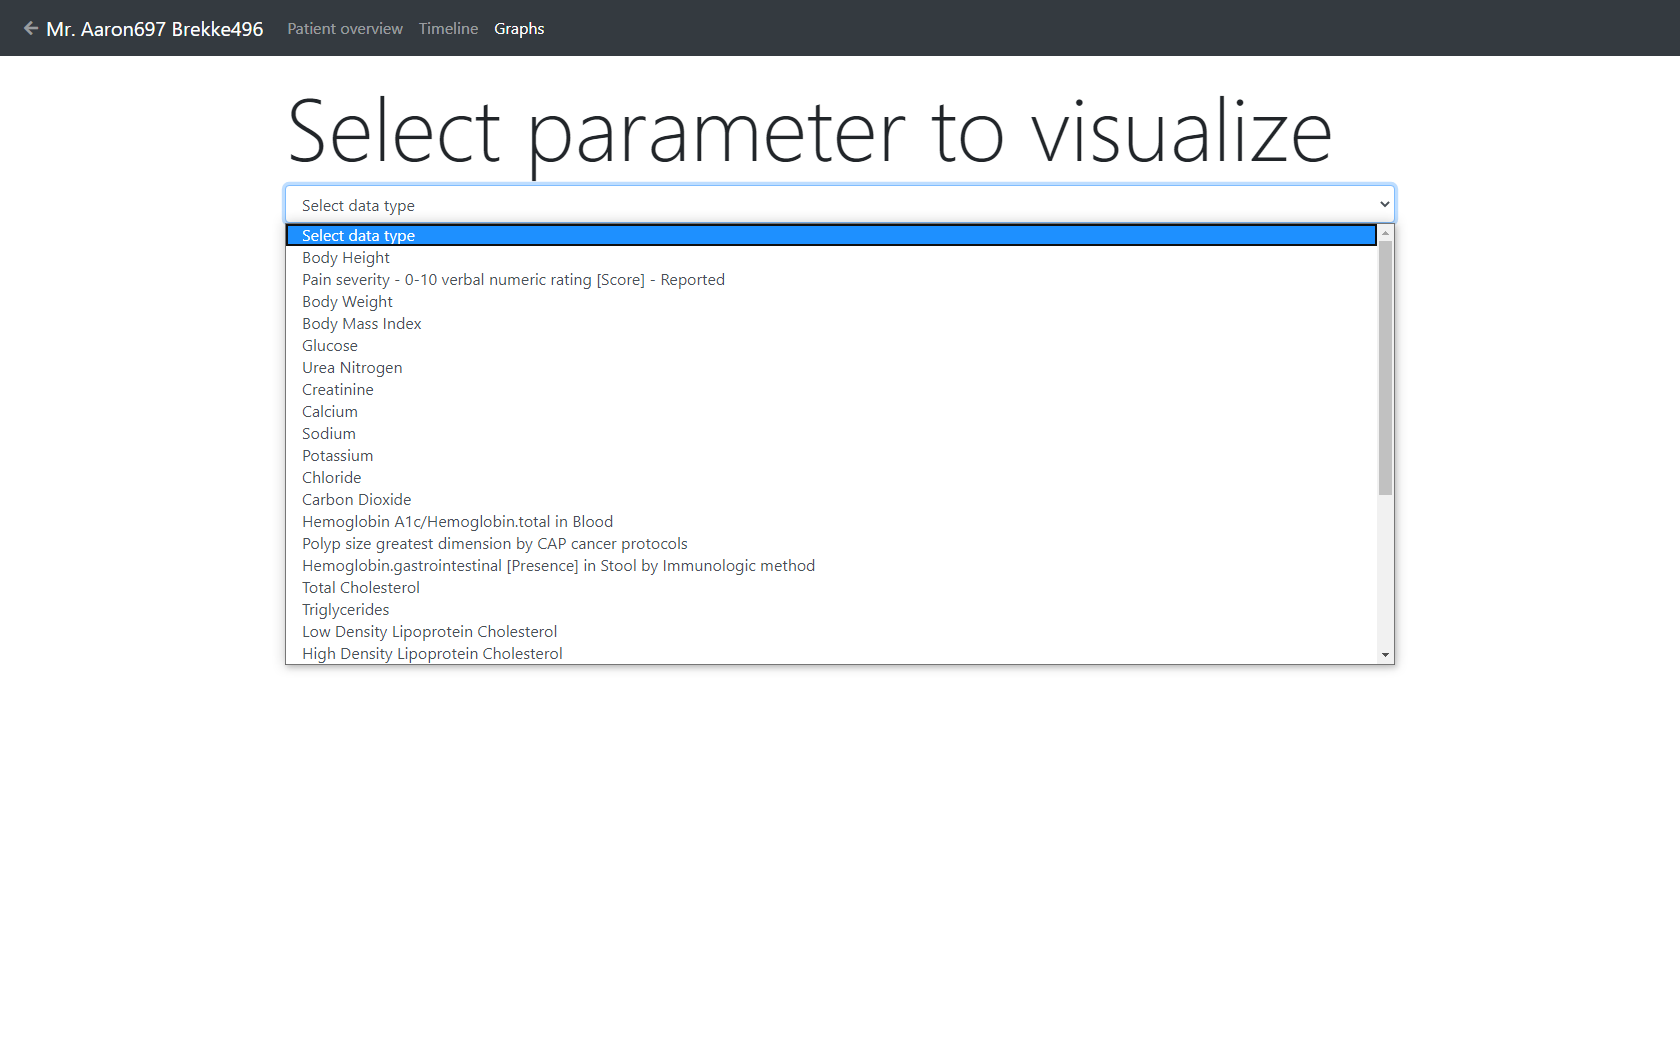
\includegraphics[width=0.8\linewidth]{pic/graph_select_data.PNG}}
    \caption{Wybór typu obserwacji}
\end{figure}
\begin{figure}[H]
    \center{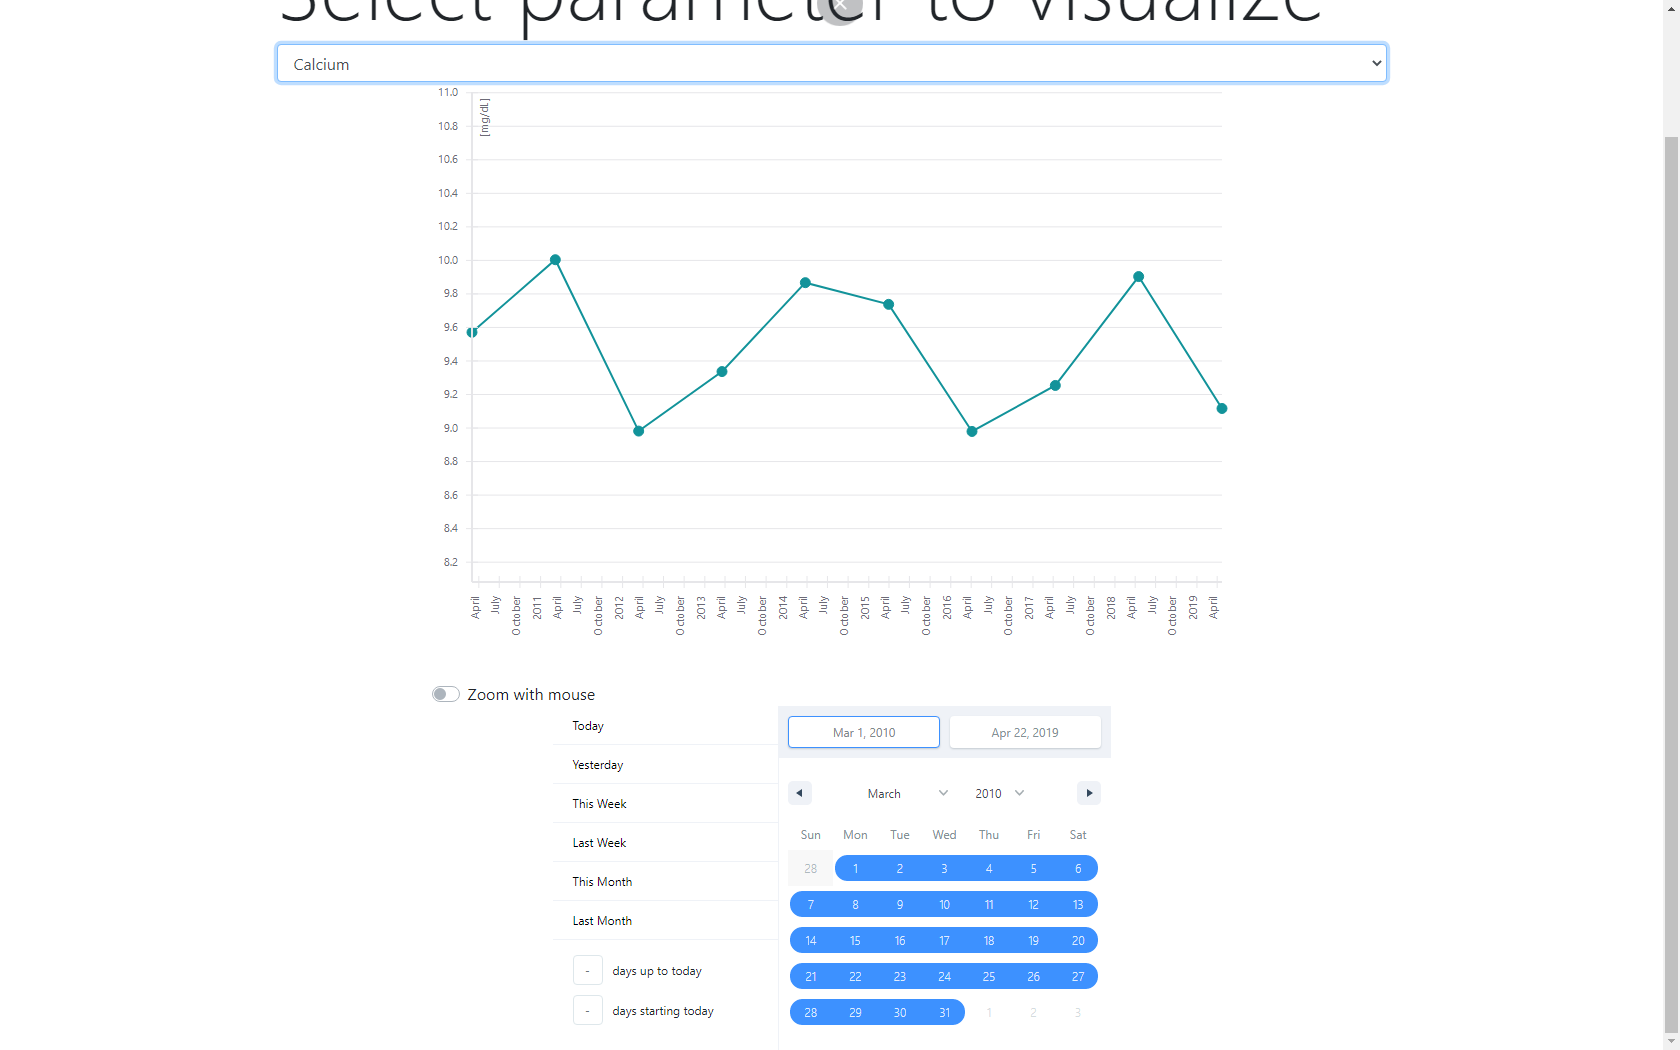
\includegraphics[width=0.8\linewidth]{pic/graph.PNG}}
    \caption{Wykres}
\end{figure}

Użytkownik może zawęzić wizualizację do wybranego przez siebie przedziału czasowego. Może tego dokonać za pomocą kalendarza 
albo zaznaczając interesujący go przedział myszą.
\begin{figure}[H]
    \center{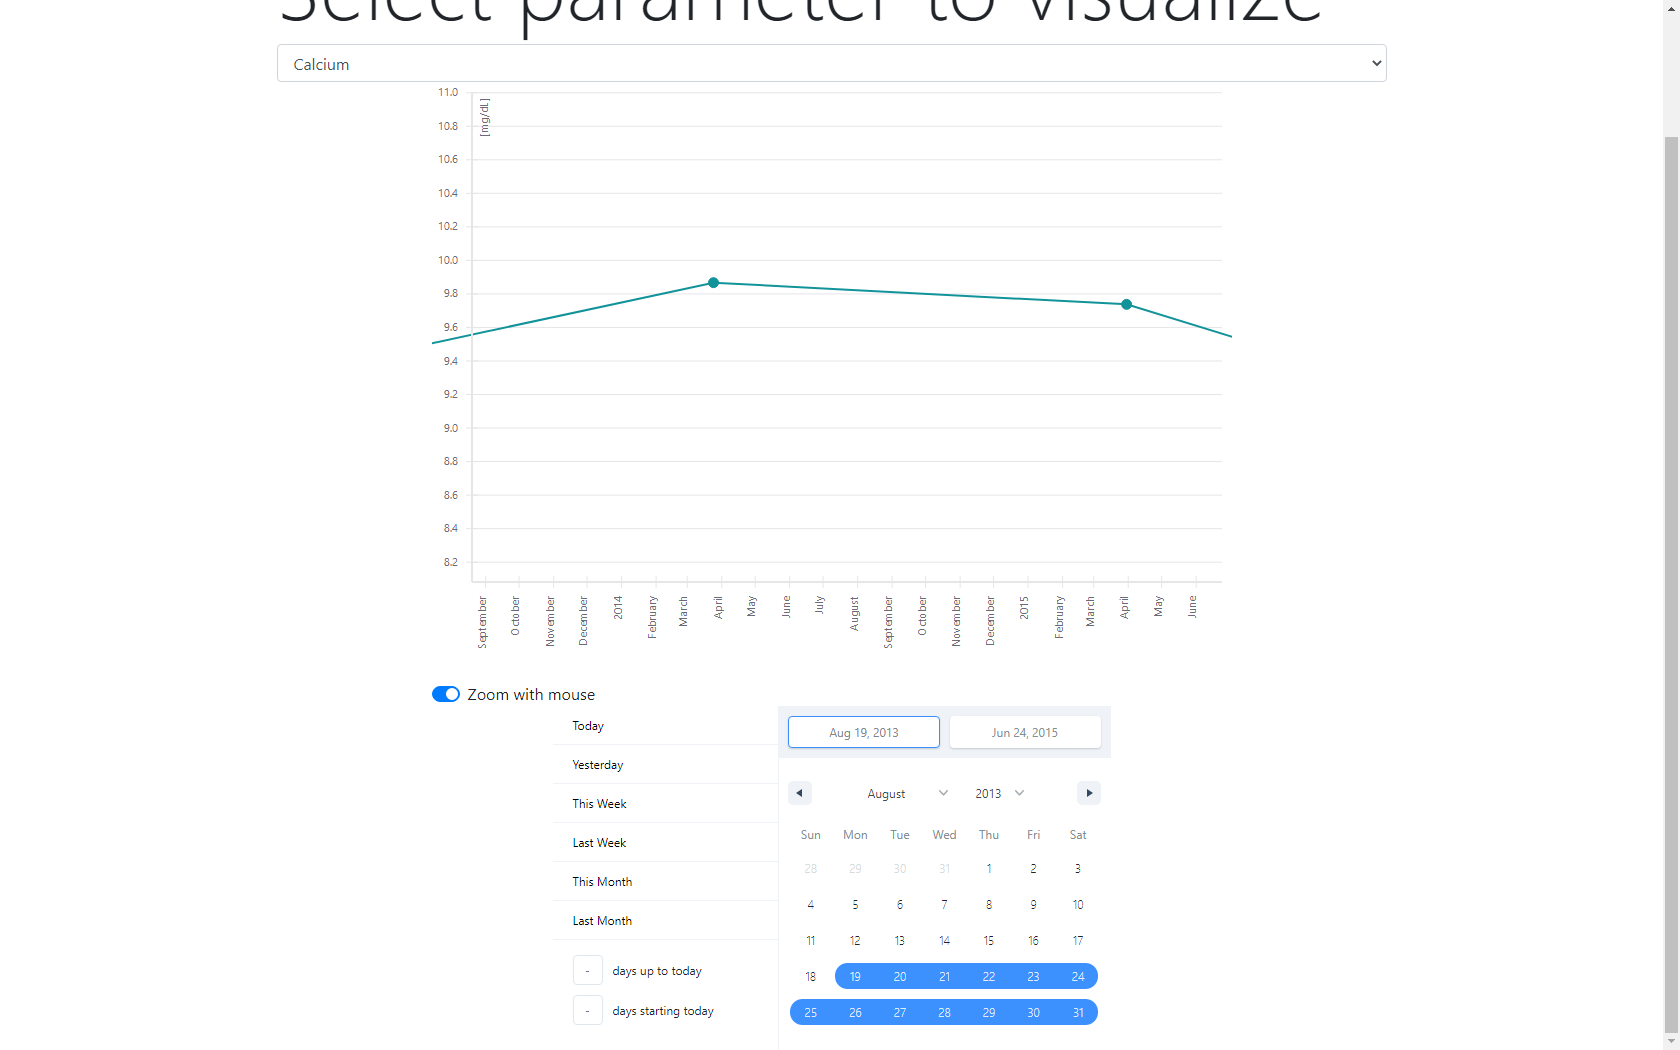
\includegraphics[width=0.8\linewidth]{pic/graph_zoomed.PNG}}
    \caption{Zawężony zakres dat na wykresie}
\end{figure}

\end{document}